\chapter{In search of solutions}\label{cap:diseño}

\section{Solving our regression problem}

The estimation of the variable \(LN\_IC\_{50}\) is considered highly beneficial in the fight against cancer. If this value can be accurately predicted, cases in which excessive medication is prescribed, potentially harming the patient's system, could be avoided. Patients requiring higher doses could be identified, thereby improving their outcomes during the course of the disease. To achieve this goal, it is essential that the target variables provided in the dataset are considered. Even if they are not all the primary objective, they can support the learning process of the algorithm, enabling more comprehensive and accurate predictions.

In line with this approach, the selected target variables, besides the \(LN\_IC\_{50}\) indicator, include the AUC curve, RMSE value, Z-Score, and the Boolean drug response. These variables contribute to understanding the behavior and characteristics of \(LN\_IC\_{50}\) across various blood samples, drugs, cancer types and other factors. Despite the preprocessing already performed, many variables still remain unordered or categorical in nature, such as blood samples, drug names or tissue descriptors. Therefore, one-hot encoding\footnote{This is a method for converting categorical data into numerical format. Instead of assigning arbitrary numeric values to categories, one-hot encoding creates a binary vector for each category \cite{amit2024onehot}.} will be applied to these features. This will be done using the get\_dummies function from the pandas library, which is already being utilized for various other operations. However, this transformation may be viewed as controversial, since it significantly increases the dataset's dimensionality, from 21 variables to 1339.

The next step to prepare the data for model training, is to divide it into three distinct subsets: a training set, a validation set and a test set. This division helps ensure that the model learns from one portion of the data the training set, while its performance is periodically evaluated on a separate subset the validation set, reducing the risk of overfitting. During training, the model attempts to minimize error on the training data, but its hyperparameters and general behavior are refined based on its performance on the validation set. Finally, once the model is fully trained, its ability to generalize is assessed using the test set, since it is a collection of data it has never seen before. This evaluation provides an unbiased estimate of the model's performance on new unseen data.

Although this step may appear straightforward, it is indispensable. It is essential to ensure that these subsets are representative of the overall data distribution. If the data is split in an unsupervised or careless manner, it may result in certain populations being excluded from the training set. This, in turn, would hinder the model's ability to learn from those data groups and ultimately reducing the generalization capacity of the model.

Therefore, after separating the data using sklearn's train\_test\_split method \cite{scikit-learn-train-test-split}, the various distributions have been represented using bar charts. This allows to check the differences between the distributions in order to detect anomalies between them.

\begin{figure}[H]
    \centering
    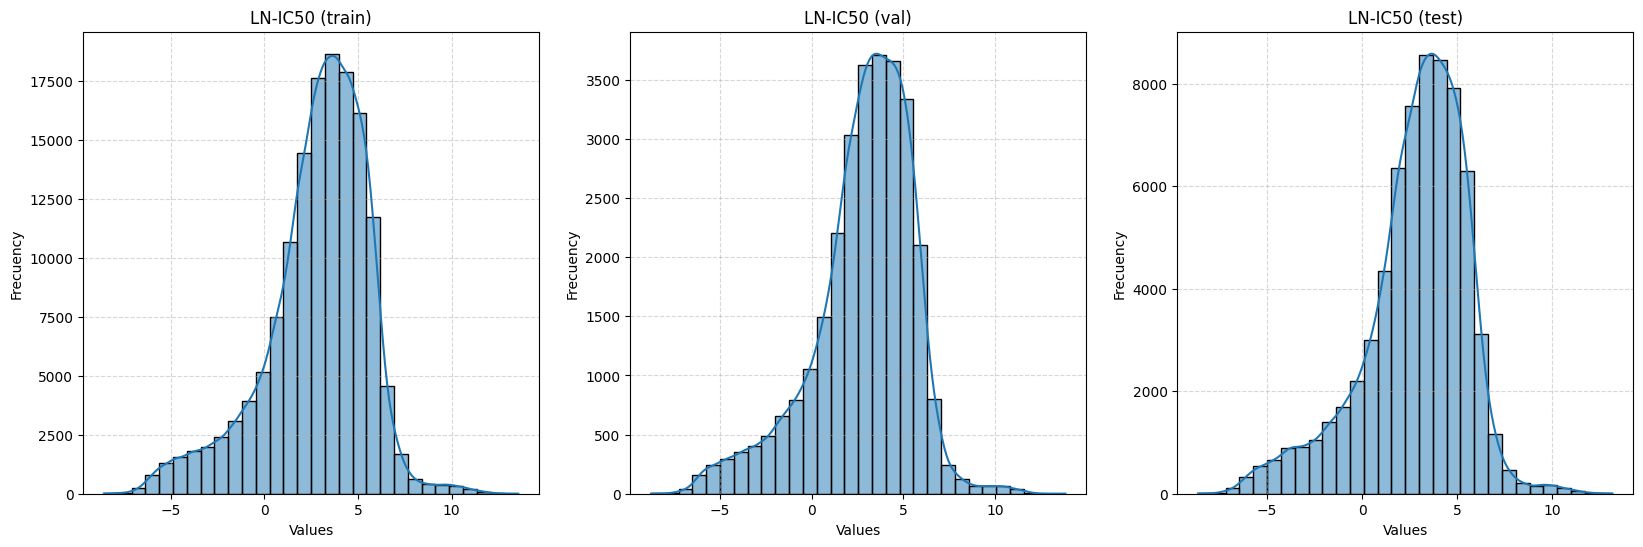
\includegraphics[width=1\textwidth]{figures/data_representation/LNIC50-splits.png}
    \caption{Distributions of the variable \(LN\_IC_{50}\) in the different subsets.}
    \label{fig:lnic50Split}
\end{figure}

\begin{figure}[H]
    \centering
    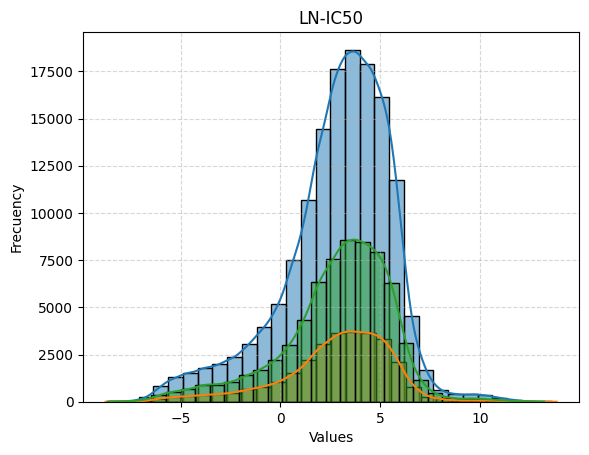
\includegraphics[width=1\textwidth]{figures/data_representation/LNIC50-splits-joined.png}
    \caption{Distributions of the variable \(LN\_IC_{50}\) in the different subsets represented in the same graph to facilitate comparison.}
    \label{fig:lnic50SplitJoined}
\end{figure}

In order to achieve better results, the data can be standarize. This process involves representing all the information on the same scale, i.e. which is specially important for algorithms like neural networks. Scikit-learn provides severals functions for this purpose, such as the StandardScaler \cite{scikit-learn-standardscaler}, which use the mean and the standar desviation to standarize the data.

The transformation applied by \texttt{StandardScaler} follows the formula:

\[
x' = \frac{x - \mu}{\sigma}
\]

Where \( x \) is the original value, \( \mu \) is the mean of the feature, and \( \sigma \) is the standard deviation.

Although the \texttt{StandardScaler} is widely used in many research studies, in this work it was decided to choose to use the \texttt{RobustScaler} \cite{scikit-learn-robustscaler} instead. This method has two main advantages: it standardizes the data while also reducing the influence of noise in the dataset. In particular, it is less sensitive to outliers, which is a highly valuable property when it is necessary to avoid misleading trends caused by extreme values. \texttt{RobustScaler} applies the formula:

\[
x' = \frac{x - \text{median}(x)}{\text{IQR}(x)}
\]

\[
\text{IQR}(x) = Q_3(x) - Q_1(x)
\]

Where \(x\) is the original value, \(x'\) is the scaled value, \(median(x)\) is the median of that feature and \(IQR\) is the interquartile range\footnote{The difference between the first and the last quartile.}. 

Given their proven effectiveness in similar contexts, both neural networks and XGBoost are selected as candidate algorithms for model training.
\begin{itemize}
    \item \textbf{Neural networks}: Neural networks are well-suited for handling high-dimensional data and typically outperform other algorithms in such contexts. In addition, applying convolutional layers could improve this predictive performance, by capturing local patterns or dependencies between related samples. This is particulary relevant, as the main aim to uncover potential relationships between blood samples, the drugs and the cancer react.
    \item \textbf{XGBoost}: Tree based model used to get great performance with tabular data, even they are able to overcome or match deep learning algorithms, like neural networks \cite{treesOverNets}. Moreover, training a tree-based model is typically faster and easier, compared to training a neural network, which takes more time. Another key advantage is interpretability, as tree models provide clearer insights into decision-making processes. However, they have one notable disadvantage: they are not able to extrapolate beyond the range of the train data due to how the algorithm learn \cite{treesLimitations}.
\end{itemize}

\subsection{Predicting $LN\_IC_{50}$ using Neural Networks}

Tensorflow is the framework selected for this reasearch due to it provides a smooth learning curve and includes built-in tools which helps to visualize the architecture and training progress.

During this research the following callbacks\footnote{Callbacks are functions or routines that are automatically called at specific points during training, such as at the end of an epoch or after a batch. They are commonly used for tasks like saving models, early stopping, adjusting the learning rate or logging training metrics.} will be used:
\begin{itemize}
    \item PlotLossesKerasTF \cite{livelossplot}: This package allows real-time visualization of training loss and other metrics during model training.
    \item ModelCheckpoint \cite{modelcheckpoint}: This callback save the best-performing model based on a chosen evaluation metric.
    \item EarlyStopping \cite{earlystopping}: Sometimes the model is not able to learn more. In this situations is common that the validation loss does not improve. When the moment in captured, the training is stopped using this callback. This enables to reduce the training time and to avoid overfitting. There are some occasions, where the model is not able to improve the validation results after a few epochs. In order to fix this, the callback needs patience of 10 epoch.
    \item ReduceLROnPlateau \cite{reducelronplateau}: Similar to the last one, this callback point out, in case the model stop of learning. In that moment it reduces the leaning rate in order to get an improvement in validation results. The patience considered was 7, as when this callback is applied the improvement is slower.
\end{itemize}



\subsubsection{Comparison of loss functions}

One of the main hyperparameters\footnote{A configuration variable set before training, which often determines whether the model learns effectively.} that must be configured during model development is the loss function. The choice of an appropriate loss function can significantly influence the quality of the results. Therefore, a function that aligns well with the nature of the problem should be selected. In this context, three potential candidates have been considered:

\begin{itemize}
    \item \textbf{MSE \cite{tensorflow-mse} (Mean Squared Error)}: Measures the averages squared difference between predicted values \(\hat{y}\) and the real ones \(y\). It is sensitive to large errors, but also to outliers. Sice the units are sqaured is less interpretable than other metrics like RMSE \cite{tensorflow-rmse}.
    \[
    \text{MSE} = \frac{1}{n} \sum_{i=1}^{n} (y_i - \hat{y}_i)^2
    \]

    \item \textbf{logCosh \cite{tensorflow-logcosh}}: It combines the best of MSE and MAE \cite{tensorflow-mae}, it is les sensitive to outliers and smoother than MAE. This function follows the formula:
    \[
    \text{LogCosh}(y, \hat{y}) = \sum_{i=1}^{n} \log\left( \cosh(\hat{y}_i - y_i) \right)
    \]

    This means in small errors it works like MSE and in the large ones, it grows more slowly like MAE. In addtion, it is derivable in all his domain, which ideal for neural network training.

    \item \textbf{Huber \cite{tensorflow-huber}}: This loss function try to replicate the principes of LogCosh, it works as squared error when this one is low, and it is linear for large errors. It requires tunning one hyperparameter, \(\delta\).
    \[
    L_{\delta}(y, \hat{y}) =
    \begin{cases}
    \frac{1}{2}(y - \hat{y})^2 & \text{if } |y - \hat{y}| \leq \delta \\
    \delta \cdot (|y - \hat{y}| - \frac{1}{2} \delta) & \text{otherwise}
    \end{cases}
    \]

\end{itemize}

\subsubsection{Development of our regressor model}

In order to determine the most appropriate approach for the research, some of methods were defined to increase the dynamism of the research. These can be found in the appendix in Listing~\ref{cod:pythonGenerateNet}, \ref{cod:pythonCompileNet} and \ref{cod:pythonShowMetrics}.


By default, the RMSE will be displayed during our training, just to interpret the learning progress.

\subsubsection{Getting the tools to compare error functions}

The initial training was conducted using Mean Squared Error (MSE) as the loss function. While simple, MSE is one of the most effective metrics for gaining insight into how well the model is learning during the early stages of training.

The training progress is illustrated in Figure~\ref{fig:mse_reg_net_train}.

\begin{figure}[H]
    \centering
    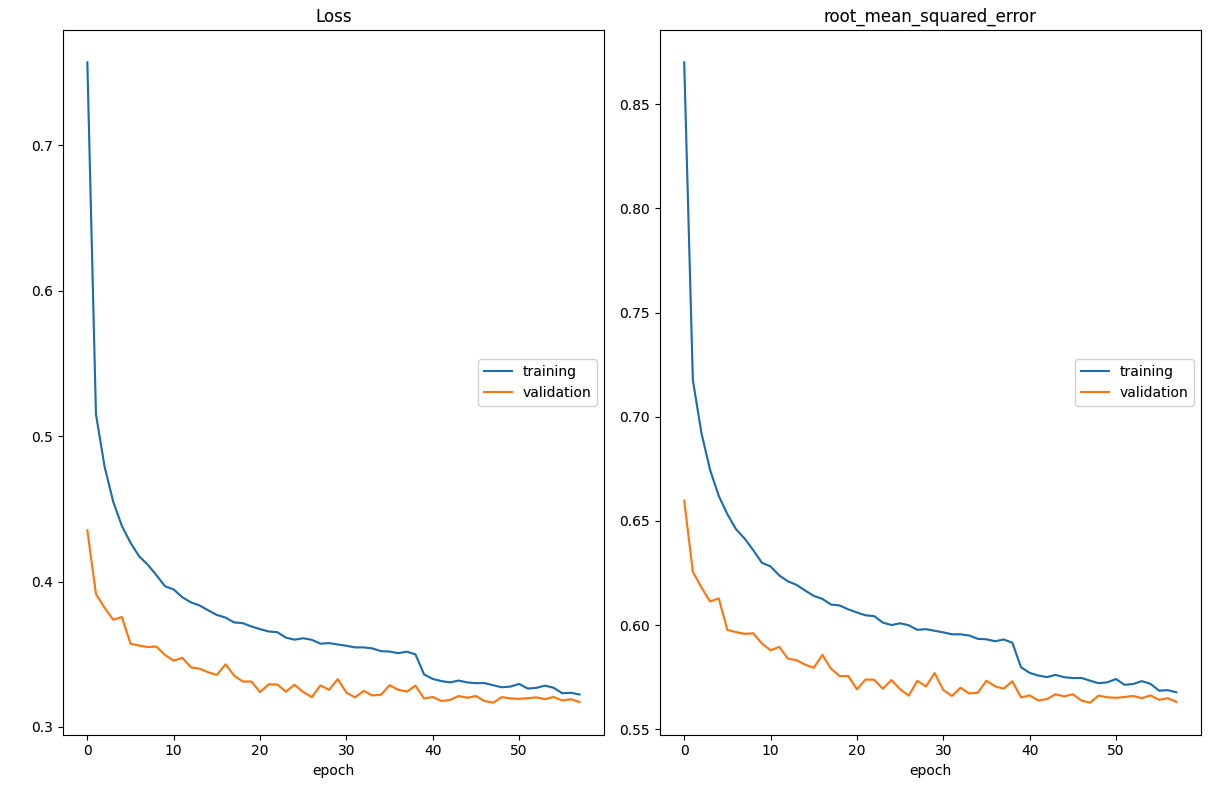
\includegraphics[width=1\textwidth]{figures/neural_net_regression_research/train_mse_neural_net.png}
    \caption{Study of the feasibility of employing MSE as a loss function using a neural network.}
    \label{fig:mse_reg_net_train}
\end{figure}

A summary of the training and validation performance, in terms of loss and RMSE, is provided in Table~\ref{tab:loss-rmse}, which shows the final values of the loss function and RMSE at the end of training.


\begin{table}[ht]
    \centering
    \begin{tabular}{|c|c|}
    \hline
    \textbf{Metric} & \textbf{Best value} \\
    \hline
    Loss (validation) & 0.317 \\
    RMSE (validation) & 0.563 \\
    \hline
    \end{tabular}
    \caption{Training and validation performance summary (loss and RMSE).}
    \label{tab:loss-rmse}
\end{table}

Finally, the overall performance of the model on the evaluation dataset is summarized in Table~\ref{tab:test_metrics_mse}:

\begin{table}[H]
    \centering
    \begin{tabular}{|c|c|}
    \hline
    \textbf{Metric} & \textbf{Value} \\
    \hline
    MSE & 0.320 \\
    RMSE & 0.566 \\
    MAE & 0.300 \\
    R\textsuperscript{2} & 0.575 \\
    \hline
    \end{tabular}
    \caption{Performance metrics on the test set using MSE as loss function.}
    \label{tab:test_metrics_mse}
\end{table}

Figure~\ref{fig:mse_reg_net_result} illustrates the relationship between the predicted values generated by our model and the corresponding actual values. In an ideal scenario, all points would lie precisely on the red diagonal line, which represents perfect predictions. Although not all predictions fall exactly on this line, the majority are closely clustered around it, indicating a generally good predictive performance. However, it is worth noting that in cases where the actual values are particularly high, the model tends to underpredict, suggesting a limitation in capturing extreme values accurately.

\begin{figure}[H]
    \centering
    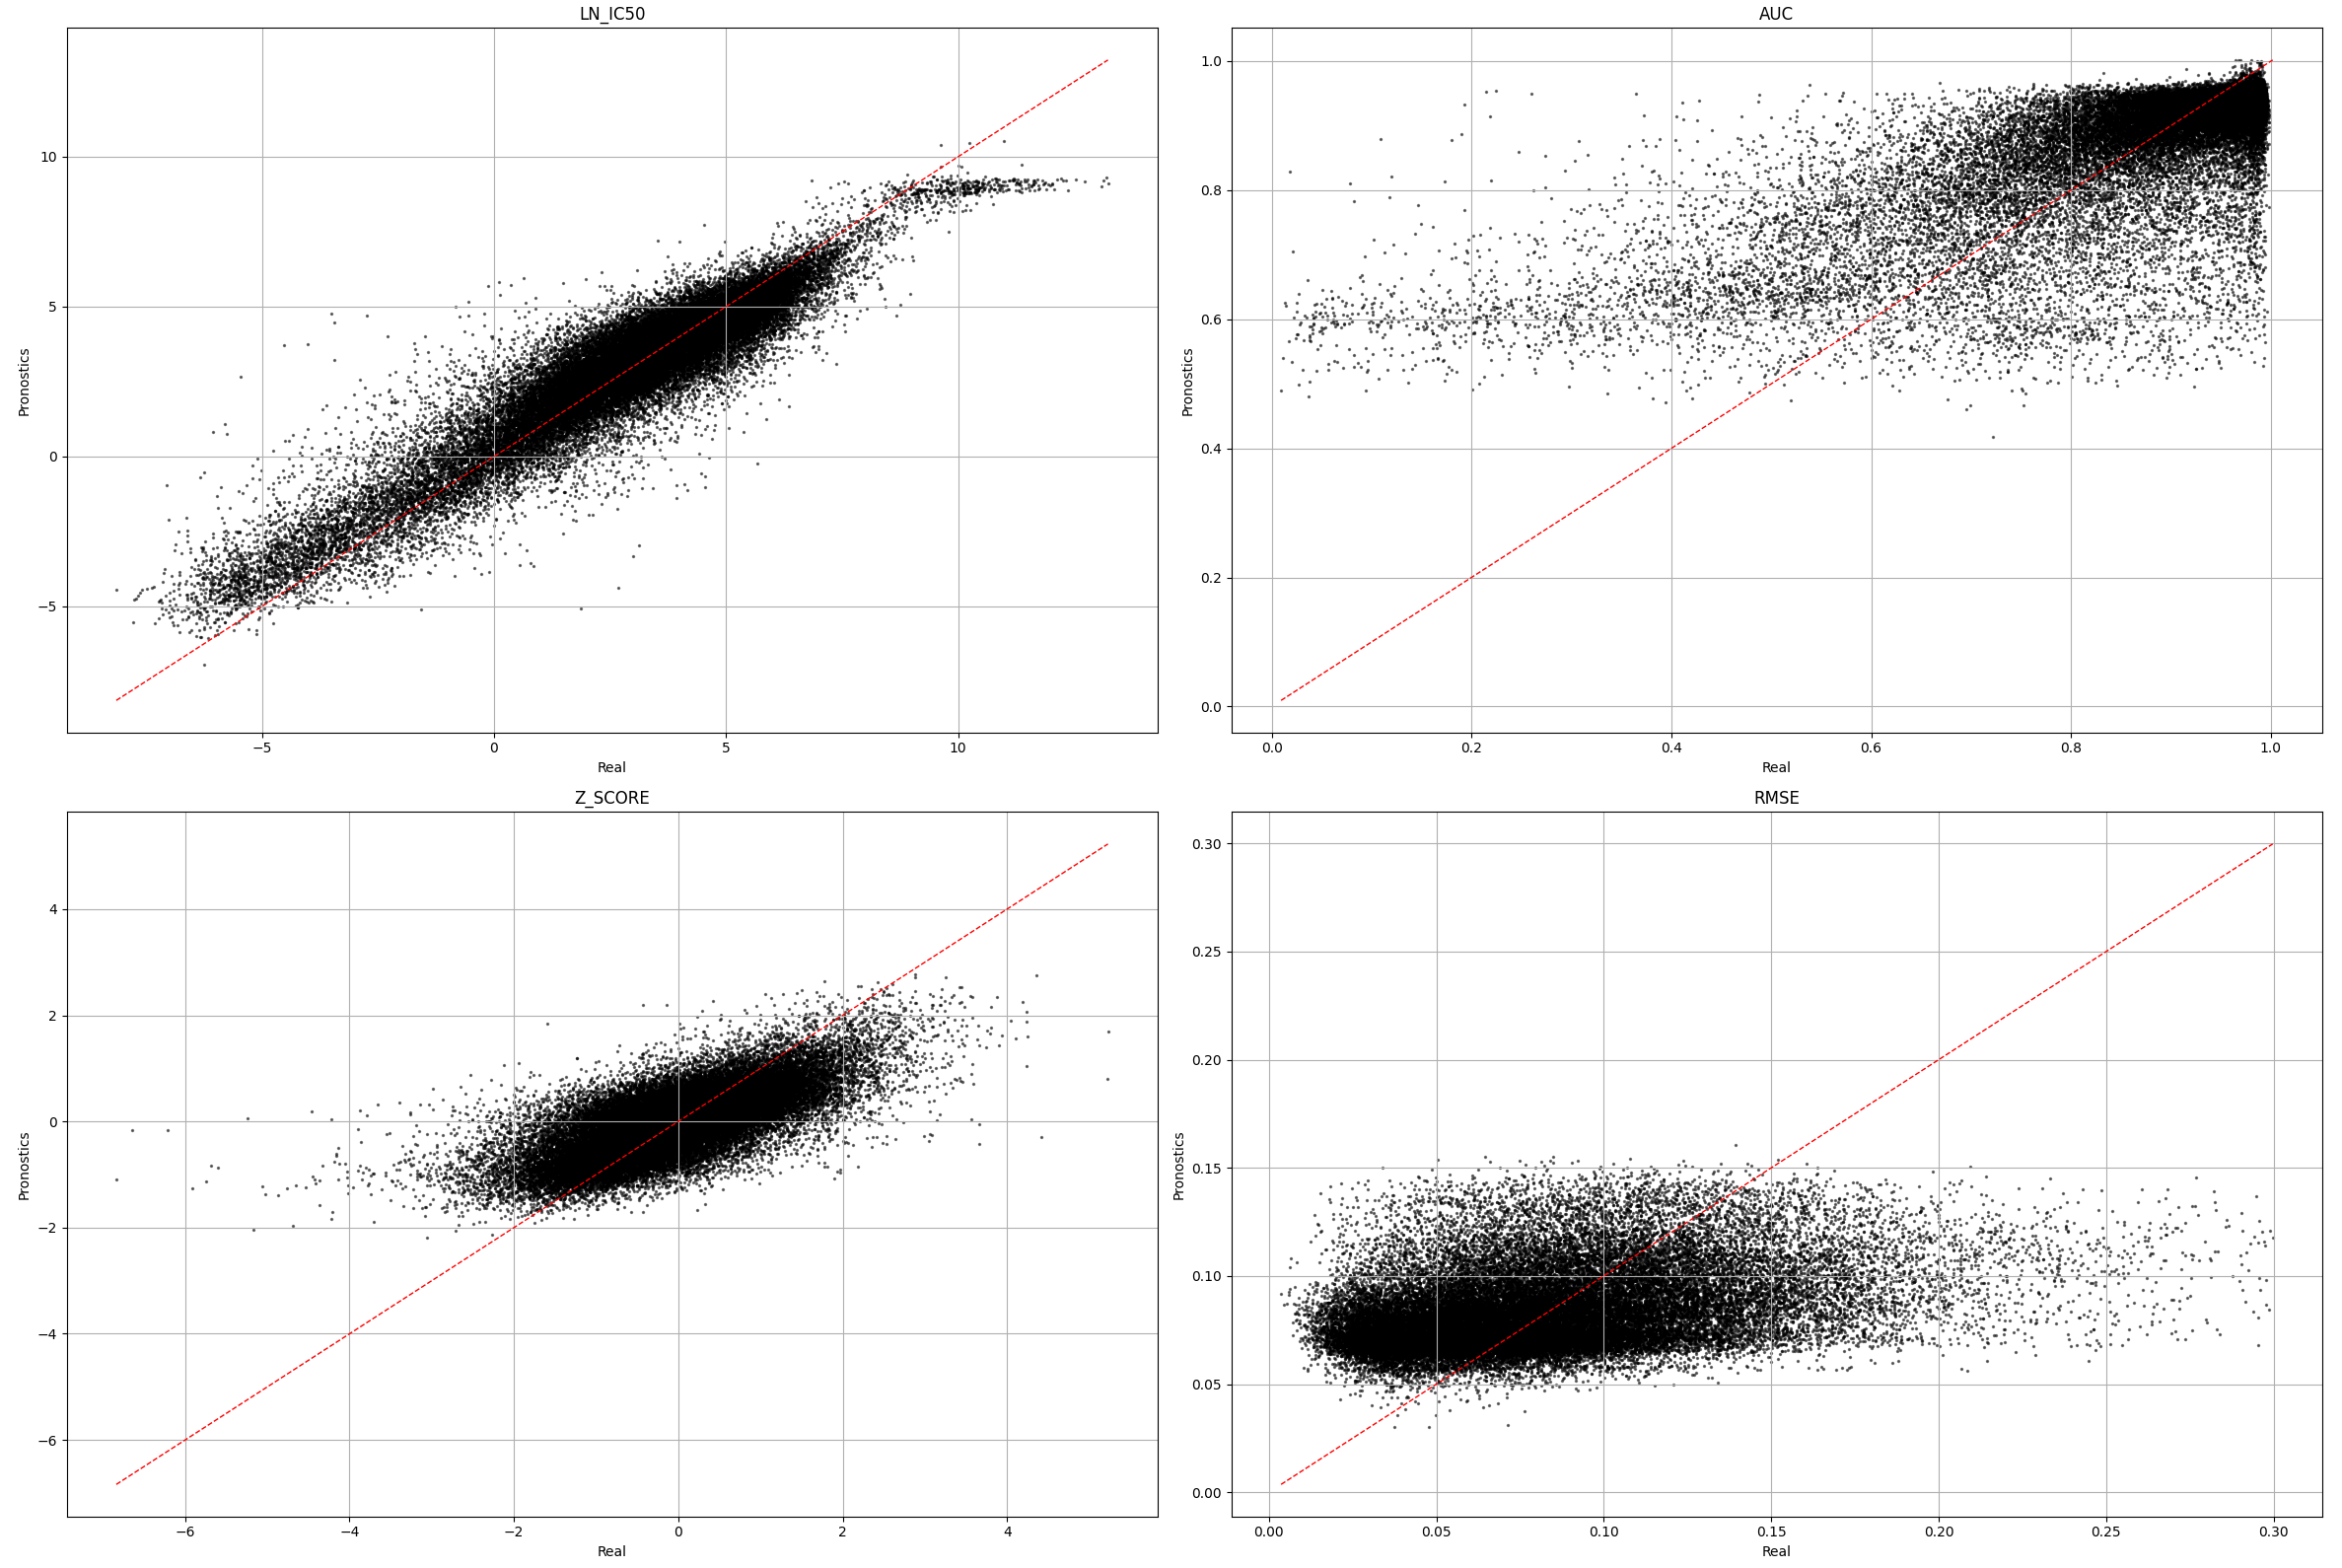
\includegraphics[width=1\textwidth]{figures/neural_net_regression_research/output_neural_net_mse.png}
    \caption{Result of employing MSE as a loss function using a neural network.}
    \label{fig:mse_reg_net_result}
\end{figure}

To further the research, the same process will be repeated with LogCosh as loss function. This could be a nice alternative because it works better with outliers than MSE and also it has a good performance with small error. For this reasons this one could be a great alternative.

In Figure~\ref{fig:logcosh_reg_net_train} si displayed the difference between training and validation, something similar to what it was seen in Figure~\ref{fig:mse_reg_net_train}. But there is a clear difference, in the previous case it seems that the model is not able to learn more, while in this one more fluctuations can be observed during learning, which allow us to see how each time the model makes a mistake and increases the error, it rectifies in the next step. This change is due to the new loss function. While ReLU is unable to represent negative values, LogCosh can. 

\begin{figure}[H]
    \centering
    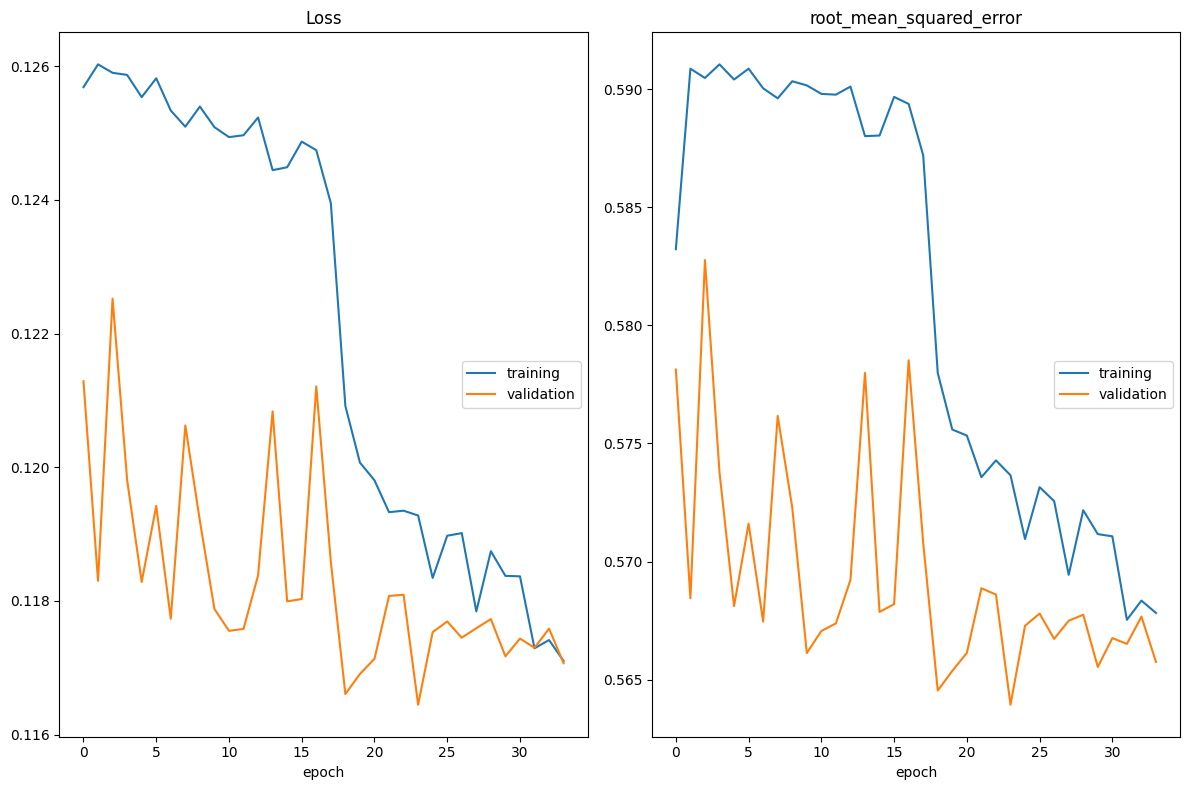
\includegraphics[width=1\textwidth]{figures/neural_net_regression_research/train_logcosh_net.png}
    \caption{Study of the feasibility of employing logarithm of the hyperbolic cosine as a loss function using a neural network.}
    \label{fig:logcosh_reg_net_train}
\end{figure}

In this case the predictions over the test set were a little bit worse that the previous one. 

\begin{table}[h]
    \centering
    \begin{tabular}{|c|c|}
    \hline
    \textbf{Metric} & \textbf{Best value} \\
    \hline
    Loss (validation) & 0.116 \\
    RMSE (validation) & 0.564 \\
    \hline
    \end{tabular}
    \caption{Validation performance metrics at the end of training using LogCosh.}
    \label{tab:loss-rmse-validation}
\end{table}

\begin{table}[H]
    \centering
    \begin{tabular}{|c|c|}
    \hline
    \textbf{Metric} & \textbf{Value} \\
    \hline
    MSE & 0.321 \\
    RMSE & 0.567 \\
    MAE & 0.299 \\
    R\textsuperscript{2} & 0.577 \\
    \hline
    \end{tabular}
    \caption{Performance metrics on the test set using LogCosh as loss function.}
    \label{tab:test_metrics_logcosh}
\end{table}

Although at first glance the results shown in Figures~\ref{fig:mse_reg_net_result} and \ref{fig:logcosh_reg_net_result} may appear nearly identical, a more in depth analysis reveals key differences. In Figure~\ref{fig:mse_reg_net_result}, the model trained with MSE appears to exhibit slightly less dispersion in its predictions, as the plot presents a more defined shape compared to that of Figure~\ref{fig:logcosh_reg_net_result}.

However, the evaluation of training progress tells a different story. In Figure~\ref{fig:mse_reg_net_train}, it can be observed that after only a few training iterations, the model reaches a plateau, showing little to no further improvement, an indication of early stagnation. In contrast, Figure~\ref{fig:logcosh_reg_net_train} displays a continued downward trend in the loss function, even in the final training stages. This suggests that the model trained with Log-Cosh loss retains the potential for further optimization, making it a more promising candidate than the one trained with MSE.


\begin{figure}[H]
    \centering
    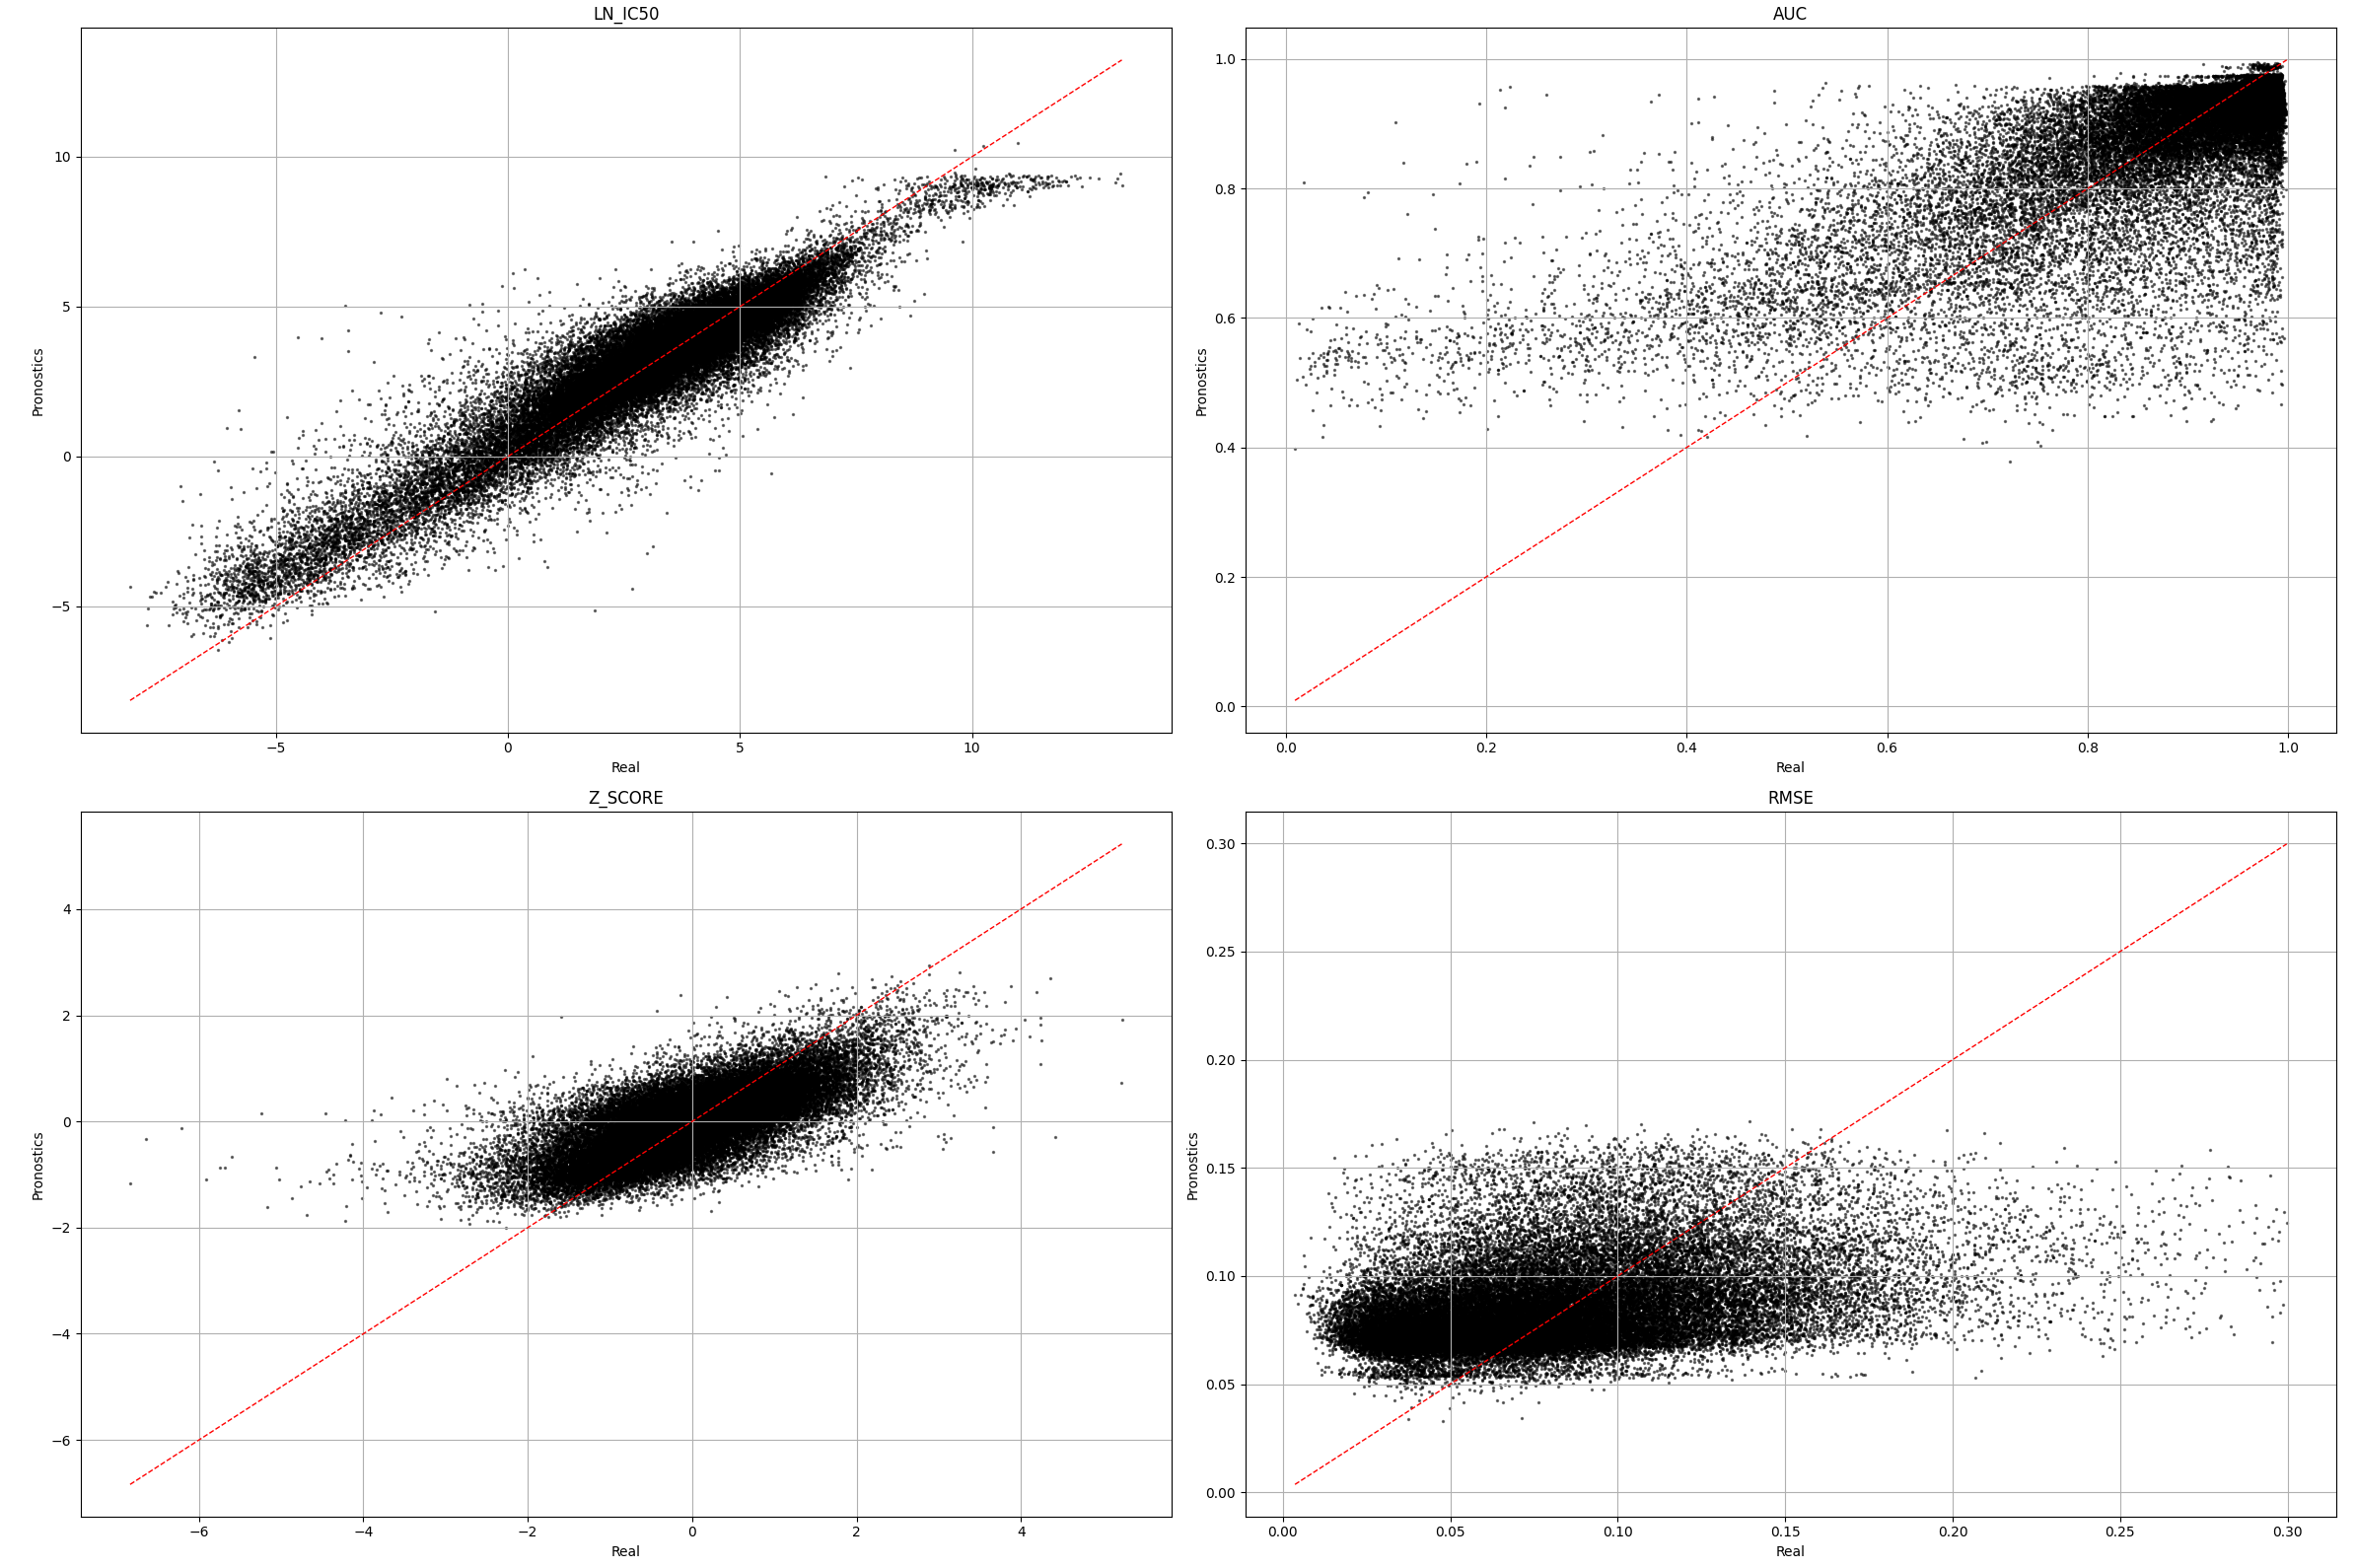
\includegraphics[width=1\textwidth]{figures/neural_net_regression_research/output_neural_net_logcosh.png}
    \caption{Result of employing logarithm of the hyperbolic cosine as a loss function using a neural network.}
    \label{fig:logcosh_reg_net_result}
\end{figure}

Finally, a new model is trained using the Huber loss function. Just as a reminder, this function and LogCosh have similar target but different points of views. The both are robust to reduce the impact of outliers, but this one require one hyperparameter, \(\delta\), which one is used as thresshold.



\begin{figure}[H]
    \centering
    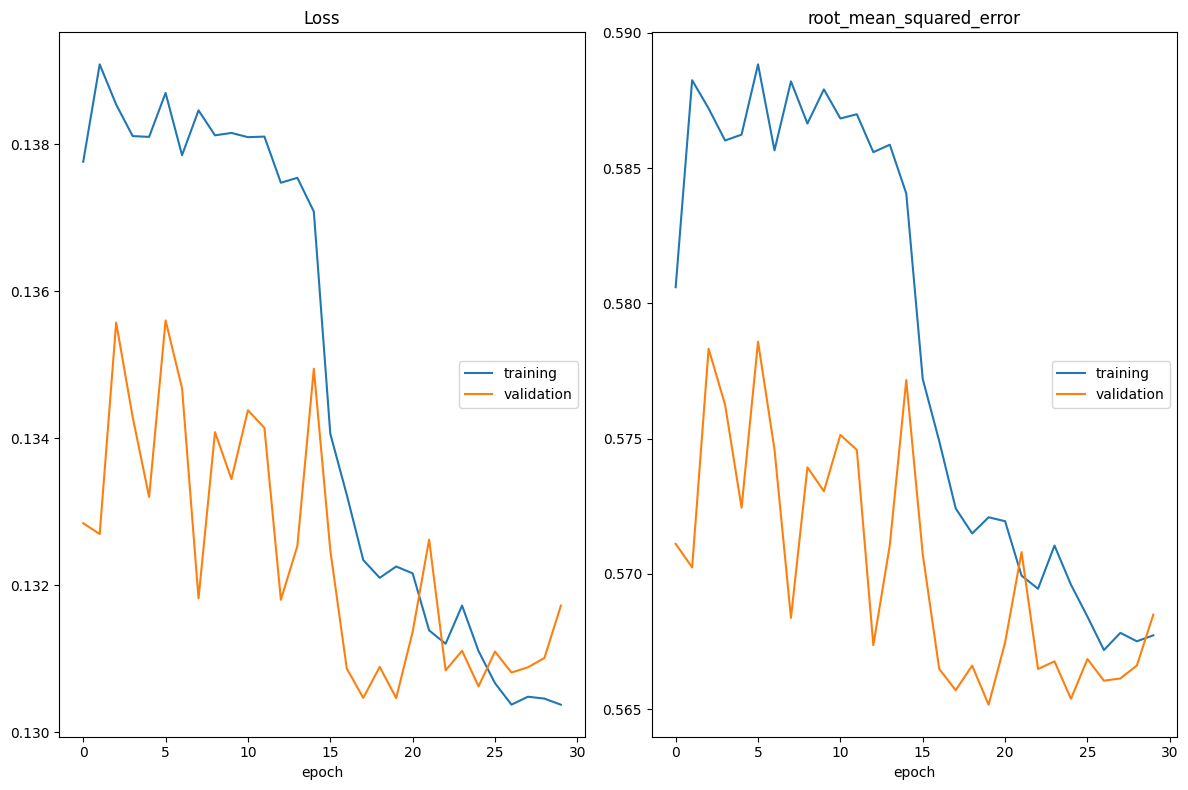
\includegraphics[width=1\textwidth]{figures/neural_net_regression_research/train_huber_net.png}
    \caption{Study of the feasibility of employing Huber as a loss function using a neural network.}
    \label{fig:huber_reg_net_train}
\end{figure}

\begin{table}[h]
    \centering
    \begin{tabular}{|c|c|}
    \hline
    \textbf{Metric} & \textbf{Best value} \\
    \hline
    Loss (validation)  & 0.130 \\
    RMSE (validation)  & 0.565 \\
    \hline
    \end{tabular}
    \caption{Validation performance metrics at the end of training using Huber loss.}
    \label{tab:loss-rmse-validation-huber}
\end{table}

\begin{table}[H]
    \centering
    \begin{tabular}{|c|c|}
    \hline
    \textbf{Metric} & \textbf{Value} \\
    \hline
    MSE & 0.321 \\
    RMSE & 0.567 \\
    MAE & 0.297 \\
    R\textsuperscript{2} & 0.586 \\
    \hline
    \end{tabular}
    \caption{Performance metrics on the test set using Huber as loss function.}
    \label{tab:test_metrics}
\end{table}


At the beginning of the training, the model trained with the Huber loss function seems really interesting, since, as illustrated in Figure~\ref{fig:huber_reg_net_train}, the results on the validation set are better than on the training set, a sign that the network is able to generalise certain behaviours. However, as the epochs go by, this difference not only reduces but the validation error exceeds the train error, gradually acquiring a clear upward trend, as can be seen in the same figure. This represents a major drawback, since if the model does not acquire or loses the ability to generalise, the results provided by the model are worthless, as it is not able to understand the nature of the progression.

\begin{figure}[H]
    \centering
    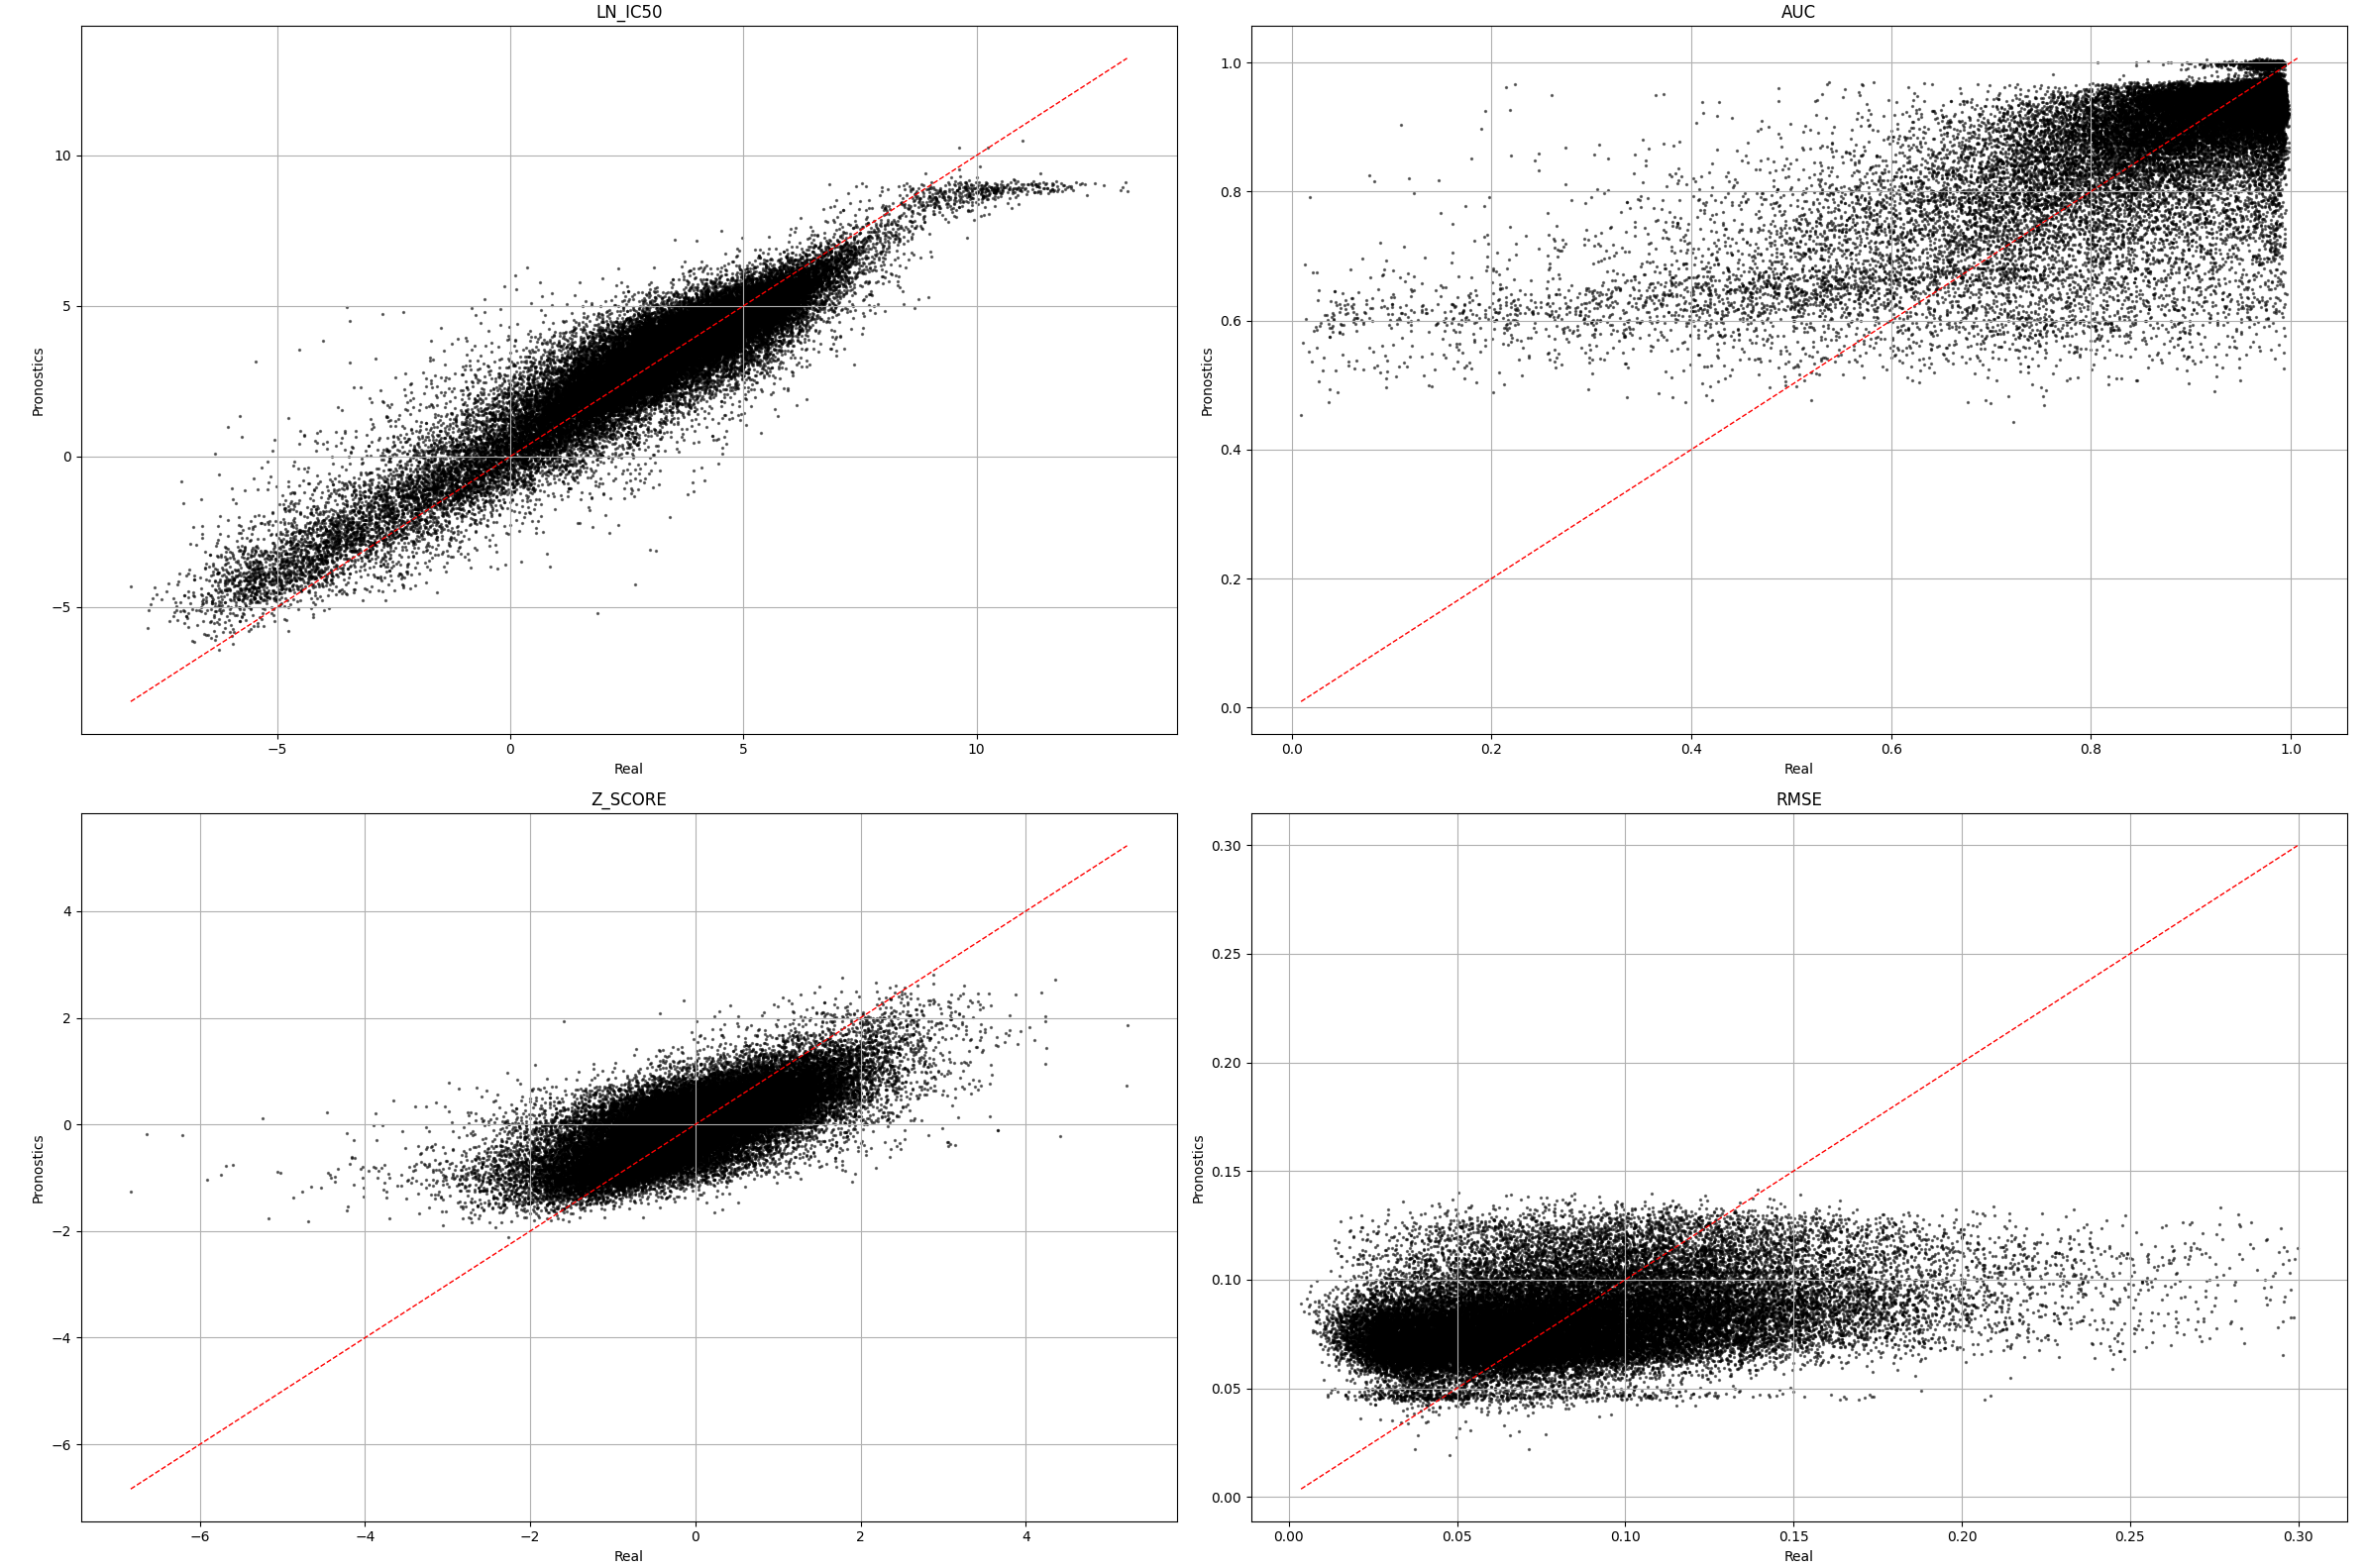
\includegraphics[width=1\textwidth]{figures/neural_net_regression_research/output_neural_net_huber.png}
    \caption{Result of employing Huber as a loss function using a neural network.}
    \label{fig:huber_reg_net_result}
\end{figure}

The three loss functions seen are interesting, as the implemented architectures that use them are able to estimate the correct form of \(LN\_IC_{50}\) in a similar way. However, this is only the beginning of defining the final model, so the best loss function will be the one that gives us a hint that it may be the start of something more promising.

Based on the results, everything seems to indicate that using the MSE error as a loss function will probably not allow us to make much progress. As previous discussed, the learning of the model that implements it does not present large variations, since the epoch 25. Only minimal improvement in validation is observed after appliying the learning rate reduction callback. 

The decision then lies between LogCosh and Huber. According to the graphs of the respective trainings, both experience oscillations in the error obtained, rectifying each time the error as the training progresses. However, as discussed in the previous analysis, Huber seems to contain an upward current from the last stage of training, while LogCosh tends to reduce the error. This is a key feature, as regularisation techniques could be used to enhance these signs of reduction and achieve a better result.

\subsubsection{Applying convolutional layers to our problem}

Once the error function has been selected, attention must be directed toward defining the architecture of the network responsible for performing the regression.

When thinking about how to organize the neurons there are many possible options, and there is no formula that indicates how to do it. So it is a trial-and-error process, with a lot of research and reading involved. Because keeping abreast of current events can save us from unnecessary testing. Something really interesting, since this type of training is not too fast.

Several studies \cite{arik2020tabnetattentiveinterpretabletabular, convolutionalToSkipImpute, tabularIntoImages} explore the use of one dimensional convolutional (1D-CNN) layers to adress problems involving tabular data. However, the effectiveness of 1D-CNN depends on the existence of a natural relationship between the variables that comprise the dataset, such as genetic sequences or cellular information. Otherwise, this type of network is not appropriate, as it may fail to capture meaningful patterns or dependencies in data lacking inherent sequential structure. In cases where the main objective is to capture local interactions between variables, 1D CNN layers represent one of the most suitable architectures that can provide meaningful insights into such relationships. This is specially significance because one of the primary goals is explain the different aspect involved in the increases or decreases of the \(LN\_IC_{50}\) variable, in order to apply that knowledge to future investigations.

After several researches \cite{softOrdering1D} is of special significance. This study iontroduce an architecture that combines a soft-ordering mechanism with 1D CNN layers to solve a regression problem, as ilustrated in Figure~\ref{fig:softOrdering1D}. To enhance performance a dense layer is first applied to the  input data to capture the spatial data or sequential relationships, without maintaining a strict order. The output is then reshape to the required dimension to allow processing through several convolutional layers. 

During the process, a branch is extranted from the initial convolutional layers. Once the main flow line passes through the last convolutional, the second flow are merged into the first one by summation, to avoid gradient vanishing. The output of this summation is subjected to average pooling and flattening before reaching the last layer, dense one as mentioned before. Finally, a dense layer performs the predictions. 

\begin{figure}[H]
    \centering
    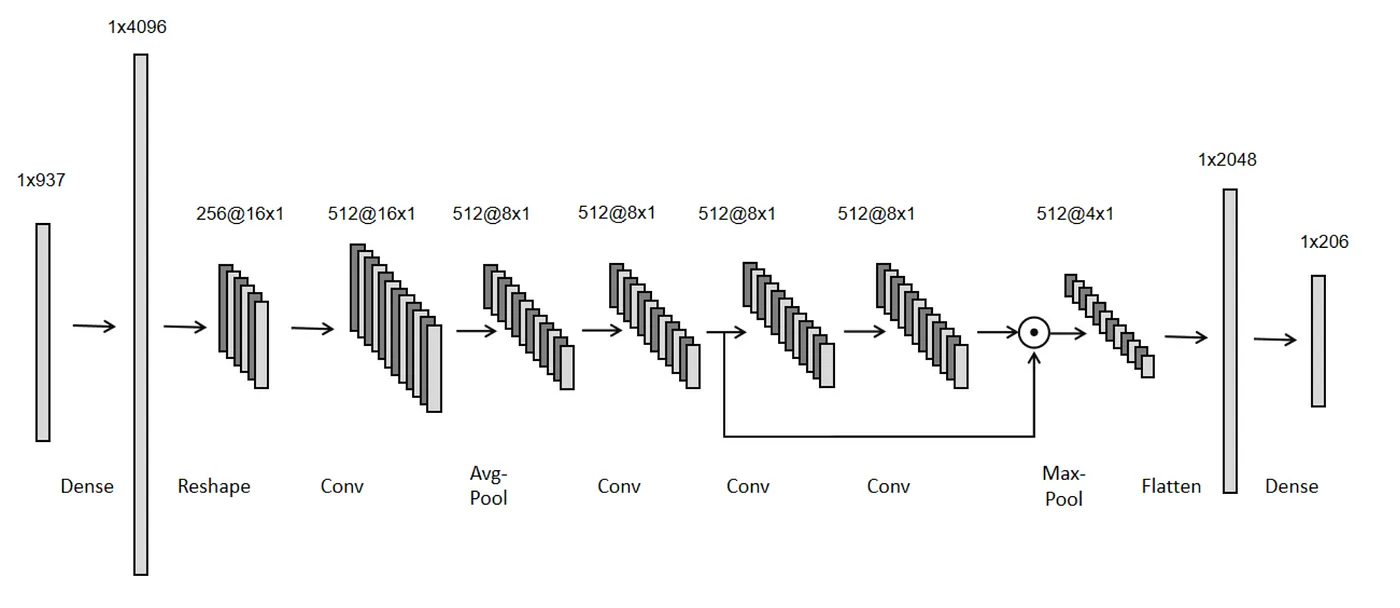
\includegraphics[width=1\textwidth]{figures/softOrdering1D.png}
    \caption{Soft-ordering with 1D convolutional architecture.}
    \label{fig:softOrdering1D}
\end{figure}

The process of reducing the error consisted of two stages. 

\begin{enumerate}
    \item Adapting the proposed architecture to the Kaggle data using tensorflow.
    \item Modifying the initial version to incorporate techniques that address issues present in the proposed dataset.
\end{enumerate}

\subsubsection{Adapting the proposed architecture to the Kaggle data using tensorflow}

The implementation was carried out using Tensorflow, based on the proposed scheme. As shown in Listing~\ref{cod:reg_addition_desbalanced}, various components from the library were utilized, such as the different types of layers, activation functions required and different regularisation techniques. This elements contributed an improvement in prediction quality, as illustrated in Figure~\ref{fig:result_addtion_reg}. In this figure, the discrepance between the predicted and actual values of the \(LN\_IC_{50}\) variable is visible reduced, indicating lower dispersion and a more accurate model, as reflected in the metrics in Table~\ref{tab:model_metrics_add_desb}. In addition, it is very important to note that Figure~\ref{fig:result_addtion_reg} no longer shows the large error that when \(LN\_IC_{50}\) variable took high values.

\begin{table}[H]
    \centering
    \begin{tabular}{|c|c|}
    \hline
    \textbf{Metric} & \textbf{Value} \\
    \hline
    Loss & 0.098 \\
    RMSE & 0.504 \\
    \hline
    \end{tabular}
    \caption{Model performance metrics on the test set during the architecture adapting phase.}
    \label{tab:model_metrics_add_desb}
\end{table}

Despite improved results, it is still possible to achieve a better quality model.

To identify potential improvements to the model, it is important to analyze Figure~\ref{fig:train_addtion_reg}, which illustrates the evolution of the loss function during training. As shown in the figure, the model initially exhibits high error, which progressively decreases as it learns to adjust its parameters. At a certain point, the loss drops significantly, suggesting that the model begins to generalize key patterns relevant to the regression task. However, this improvement plateaus after a few iterations, with no further reduction in error.

Moreover, a considerable gap is observed between the training and validation errors, with the training loss being significantly lower. This discrepancy suggests that, although there is no clear indication of overfitting, the model performs considerably better on the training set than on the validation set. This implies that it may not be capturing generalizable patterns well enough to accurately predict unseen data. Reducing this gap could therefore help to achieve better results.

\begin{figure}[H]
    \centering
    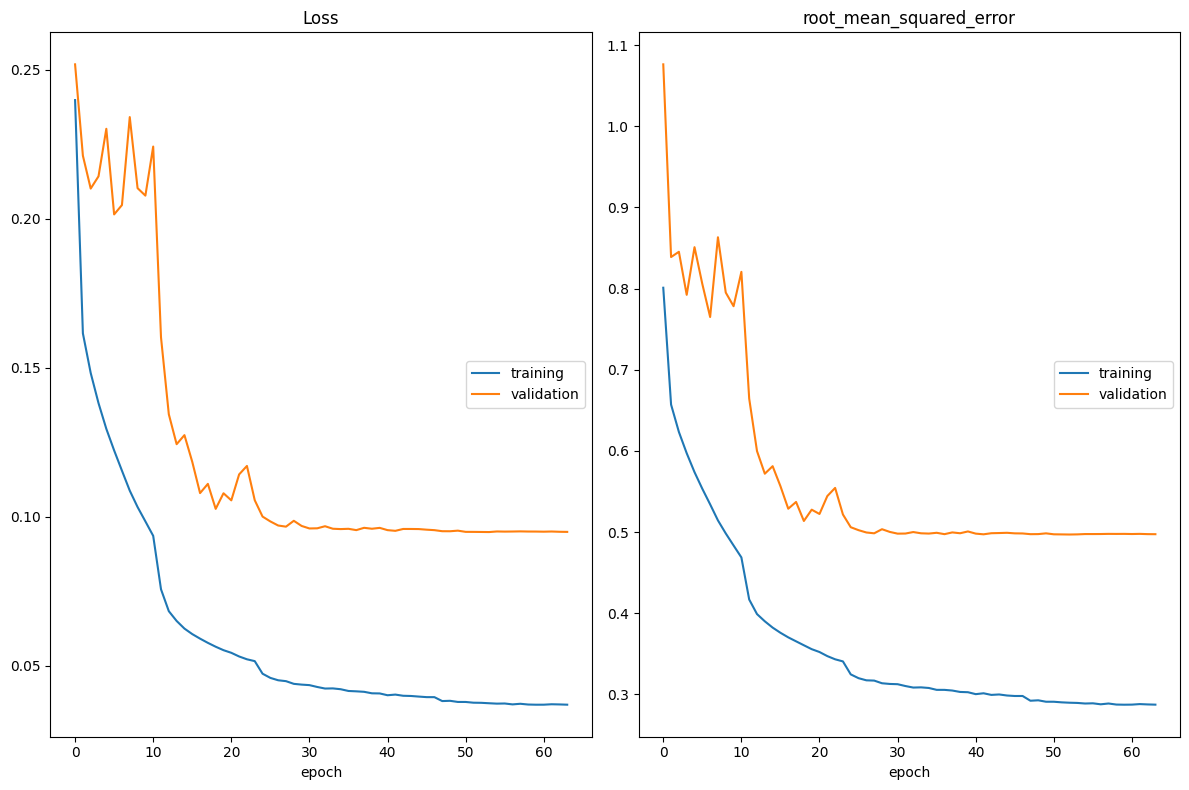
\includegraphics[width=1\textwidth]{figures/neural_net_regression_addition/train_logcosh_addition_desbalanced.png}
    \caption{Training a neural network using convolutional layers and addition as a bridge.}
    \label{fig:train_addtion_reg}
\end{figure}


\begin{figure}[H]
    \centering
    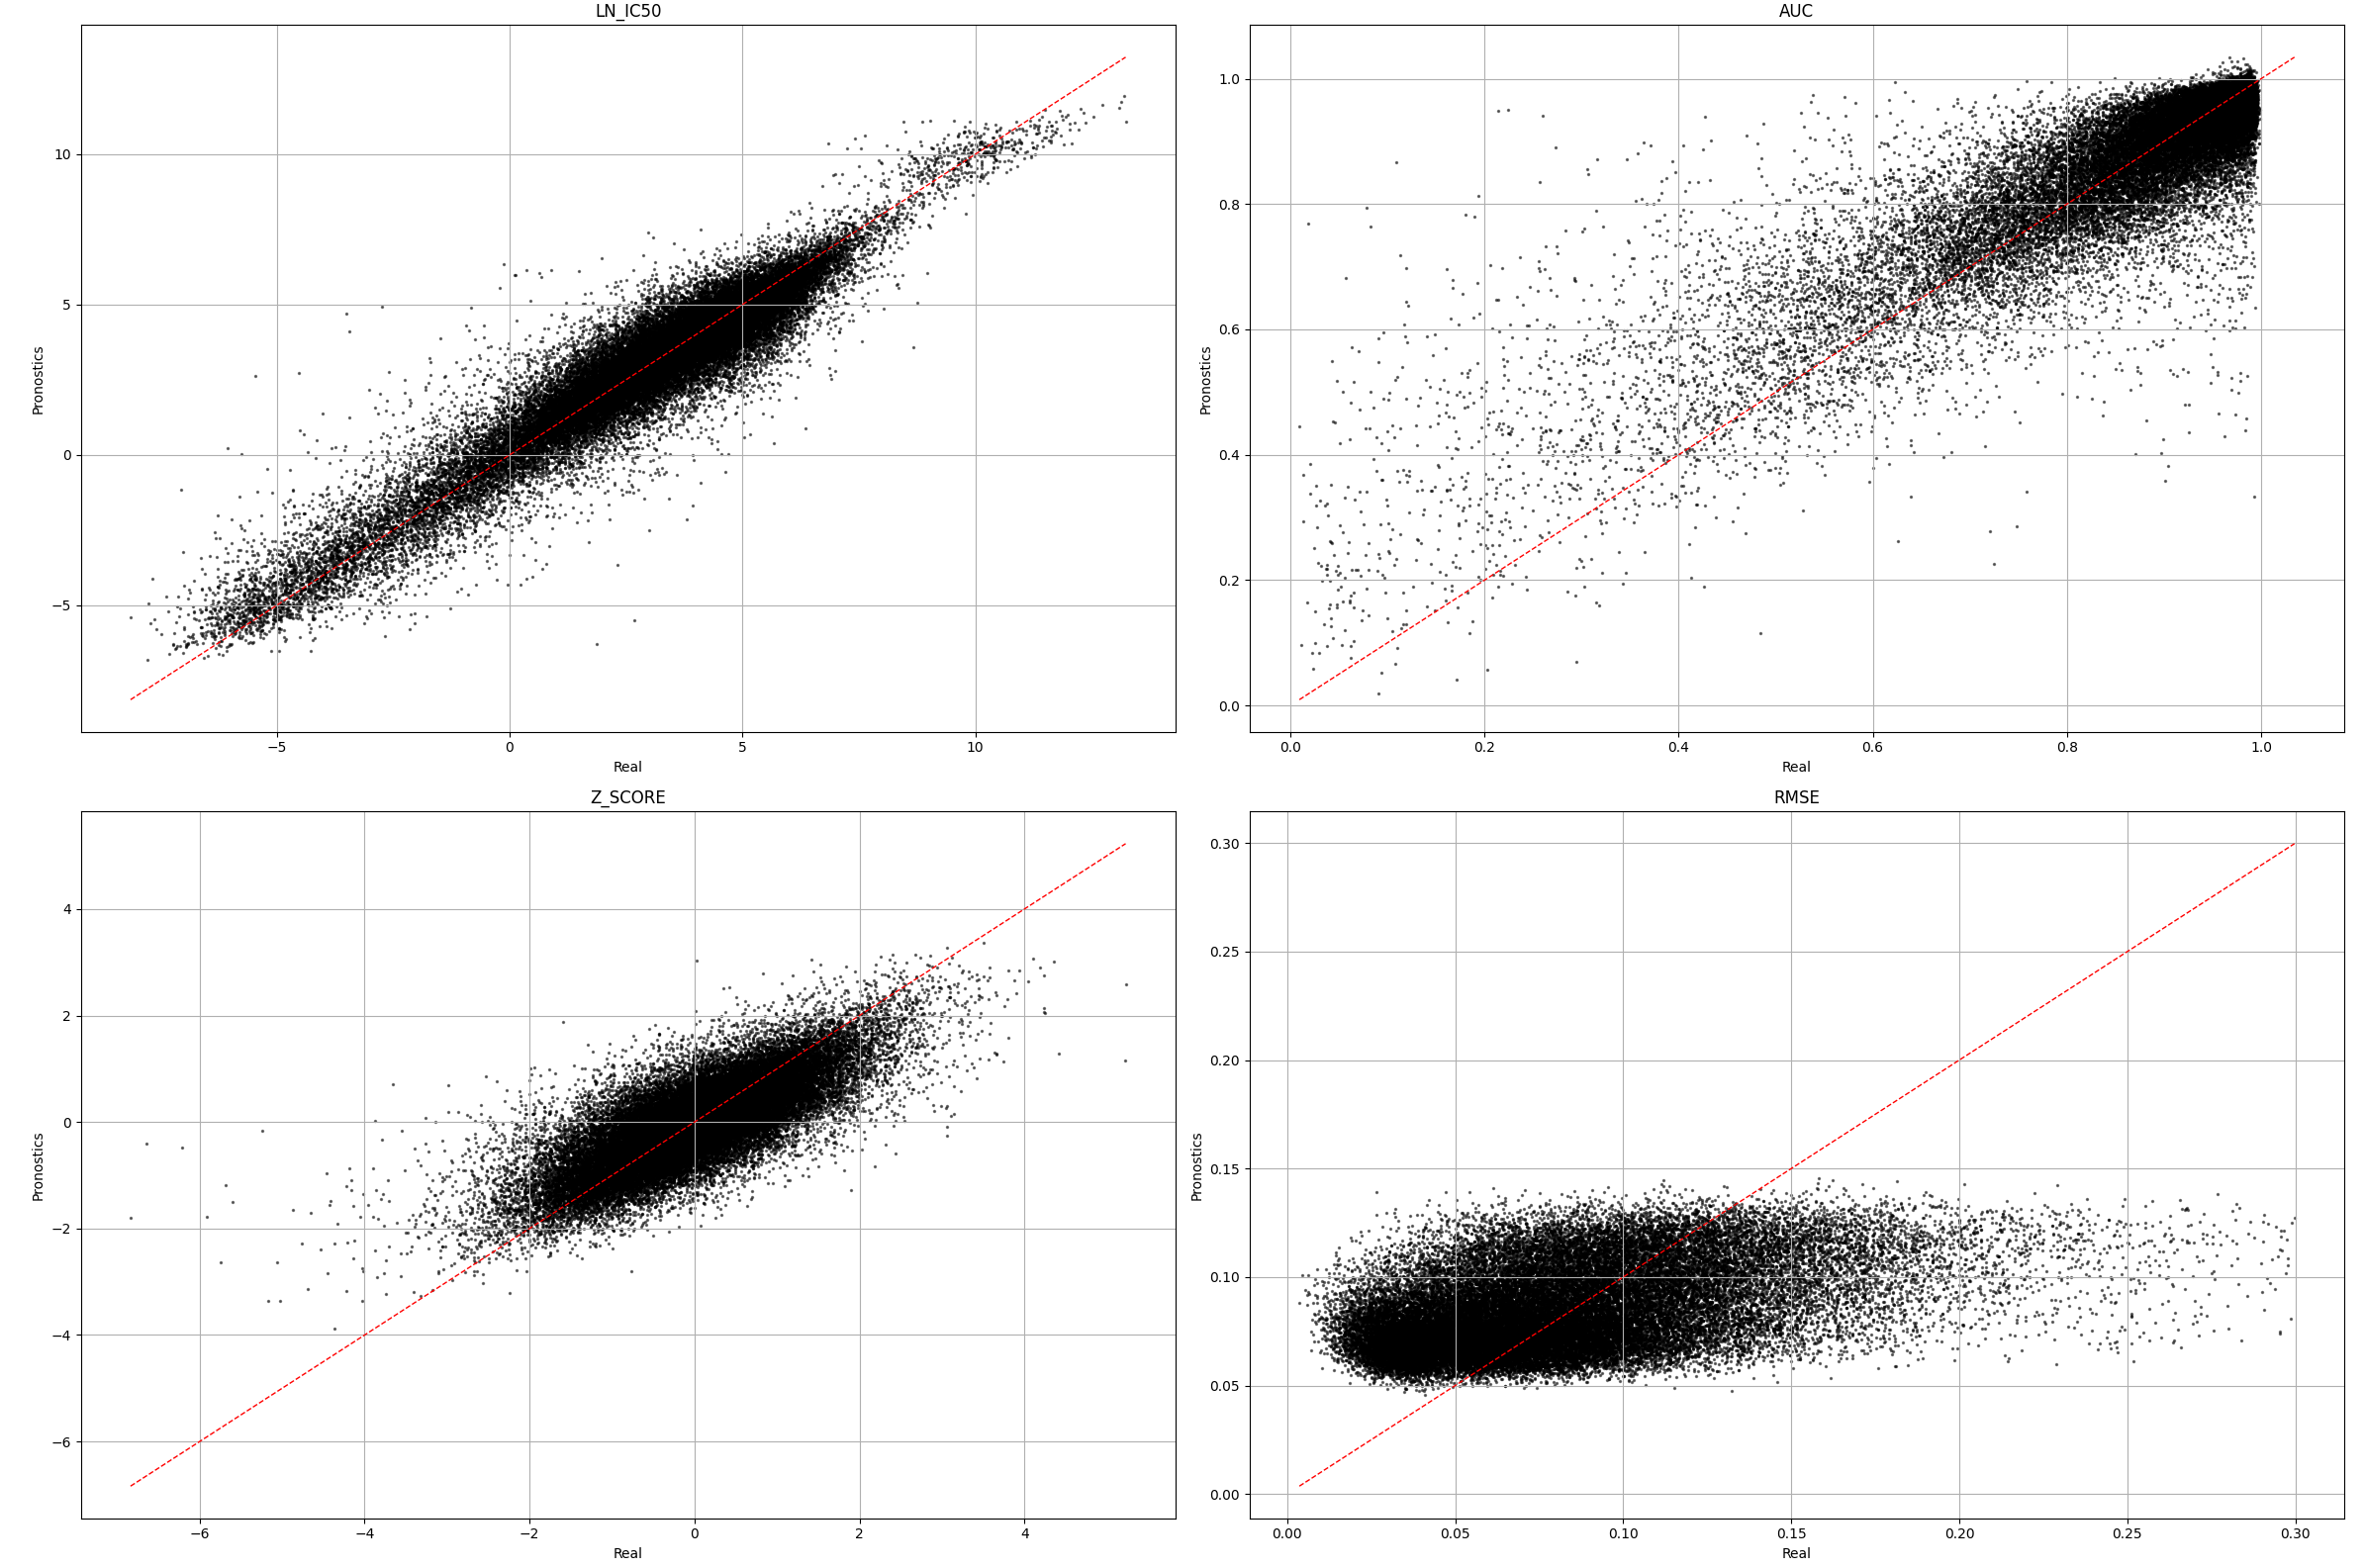
\includegraphics[width=1\textwidth]{figures/neural_net_regression_addition/output_neural_net_addition_desbalanced.png}
    \caption{Result of employing a neural network using convolutional layers and addition as a bridge.}
    \label{fig:result_addtion_reg}
\end{figure}

\subsubsection{Modifying the initial version to incorporate techniques that address issues present in the proposed dataset}

To mitigate overfitting, numerous experiments were conducted by increasing and varying different types of regularization techniques. However, the results remained largely unchanged, with only marginal improvements in error reduction. In contrast, experimenting with different activation functions led to more promising results. Initially, the functions suggested in the original paper were tested, but subsequently, other activation functions available in TensorFlow were explored. Among these, the SiLU function \cite{silu}, also known as Swish, proved particularly effective. It significantly reduced the gap between training and validation errors.

This improvement can be attributed to the characteristics of SiLU compared to ReLU and the specific nature of our dataset. SiLU is a smoother function with outputs close to zero, as illustrated in Figure~\ref{fig:compararisionSiluRelu}, making it more suitable in scenarios where small negative values may carry meaningful information. Unlike ReLU, which zeroes out all negative values, SiLU retains them with a small but non-zero output, allowing a more nuanced interpretation.

One of the main drawbacks of SiLU is its higher computational cost, as it requires computing a sigmoid function in addition to a multiplication operation. In contrast, ReLU simply computes the maximum between zero and the input value. The formula for SiLU is:

\[
\text{SiLU}(x) = x \cdot \sigma(x) = \frac{x}{1 + e^{-x}} \quad \text{where } \sigma(x) \text{ is the sigmoid function}
\]

\begin{figure}[H]
    \centering
    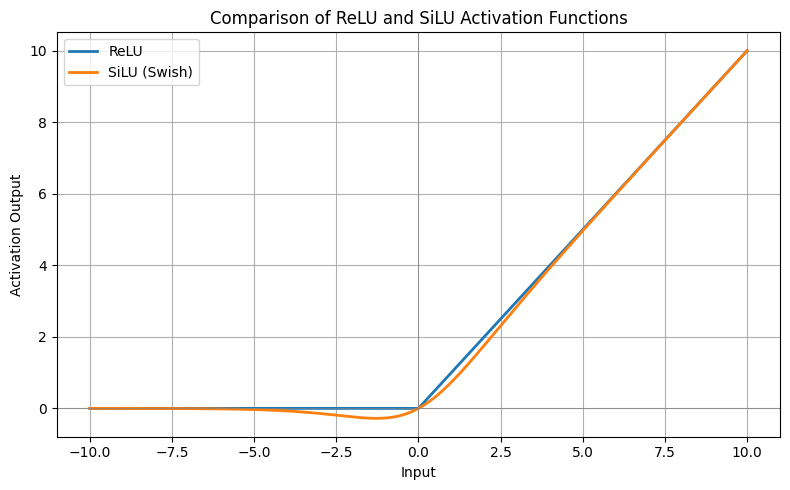
\includegraphics[width=1\textwidth]{figures/neural_net_regression_research/reluSilucomparison.png}
    \caption{ Comparision between SiLU and ReLU. In this picture it is observed the differeces between them around zero.}
    \label{fig:compararisionSiluRelu}
\end{figure}

On this basis, the implementation, shown in Listing~\ref{cod:reg_addition_balanced}, was carried out again, adjusting some of the hyperparameters related to the regularization and the number of layers. As a result of these modifications, the difference between the train and valiadation was reduced, showing a narrower gap, as is ilustrate by Figure~\ref{fig:train_addtion_reg_balanced}.

\begin{figure}[H]
    \centering
    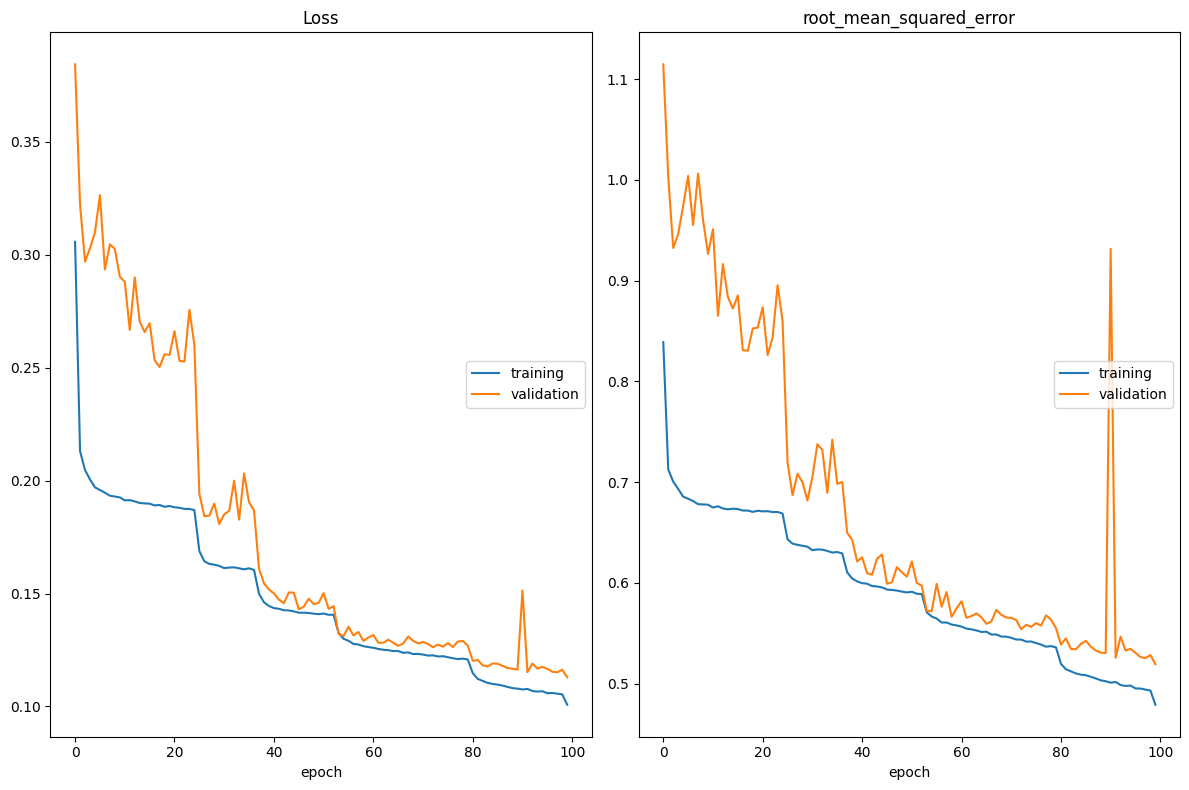
\includegraphics[width=1\textwidth]{figures/neural_net_regression_addition/train_logcosh_addition_balanced.png}
    \caption{Training a neural network using convolutional layers and addition as a bridge, increasing the regularization and using SiLU as activation function.}
    \label{fig:train_addtion_reg_balanced}
\end{figure}

\begin{table}[H]
    \centering
    \begin{tabular}{|c|c|}
    \hline
    \textbf{Metric} & \textbf{Value} \\
    \hline
    MSE & 0.270 \\
    RMSE & 0.520 \\
    MAE & 0.257 \\
    R\textsuperscript{2} & 0.685 \\
    \hline
    \end{tabular}
    \caption{Performance metrics on the test set after applying the SiLU activation function.}
    \label{tab:metrics_silu}
\end{table}

\begin{figure}[H]
    \centering
    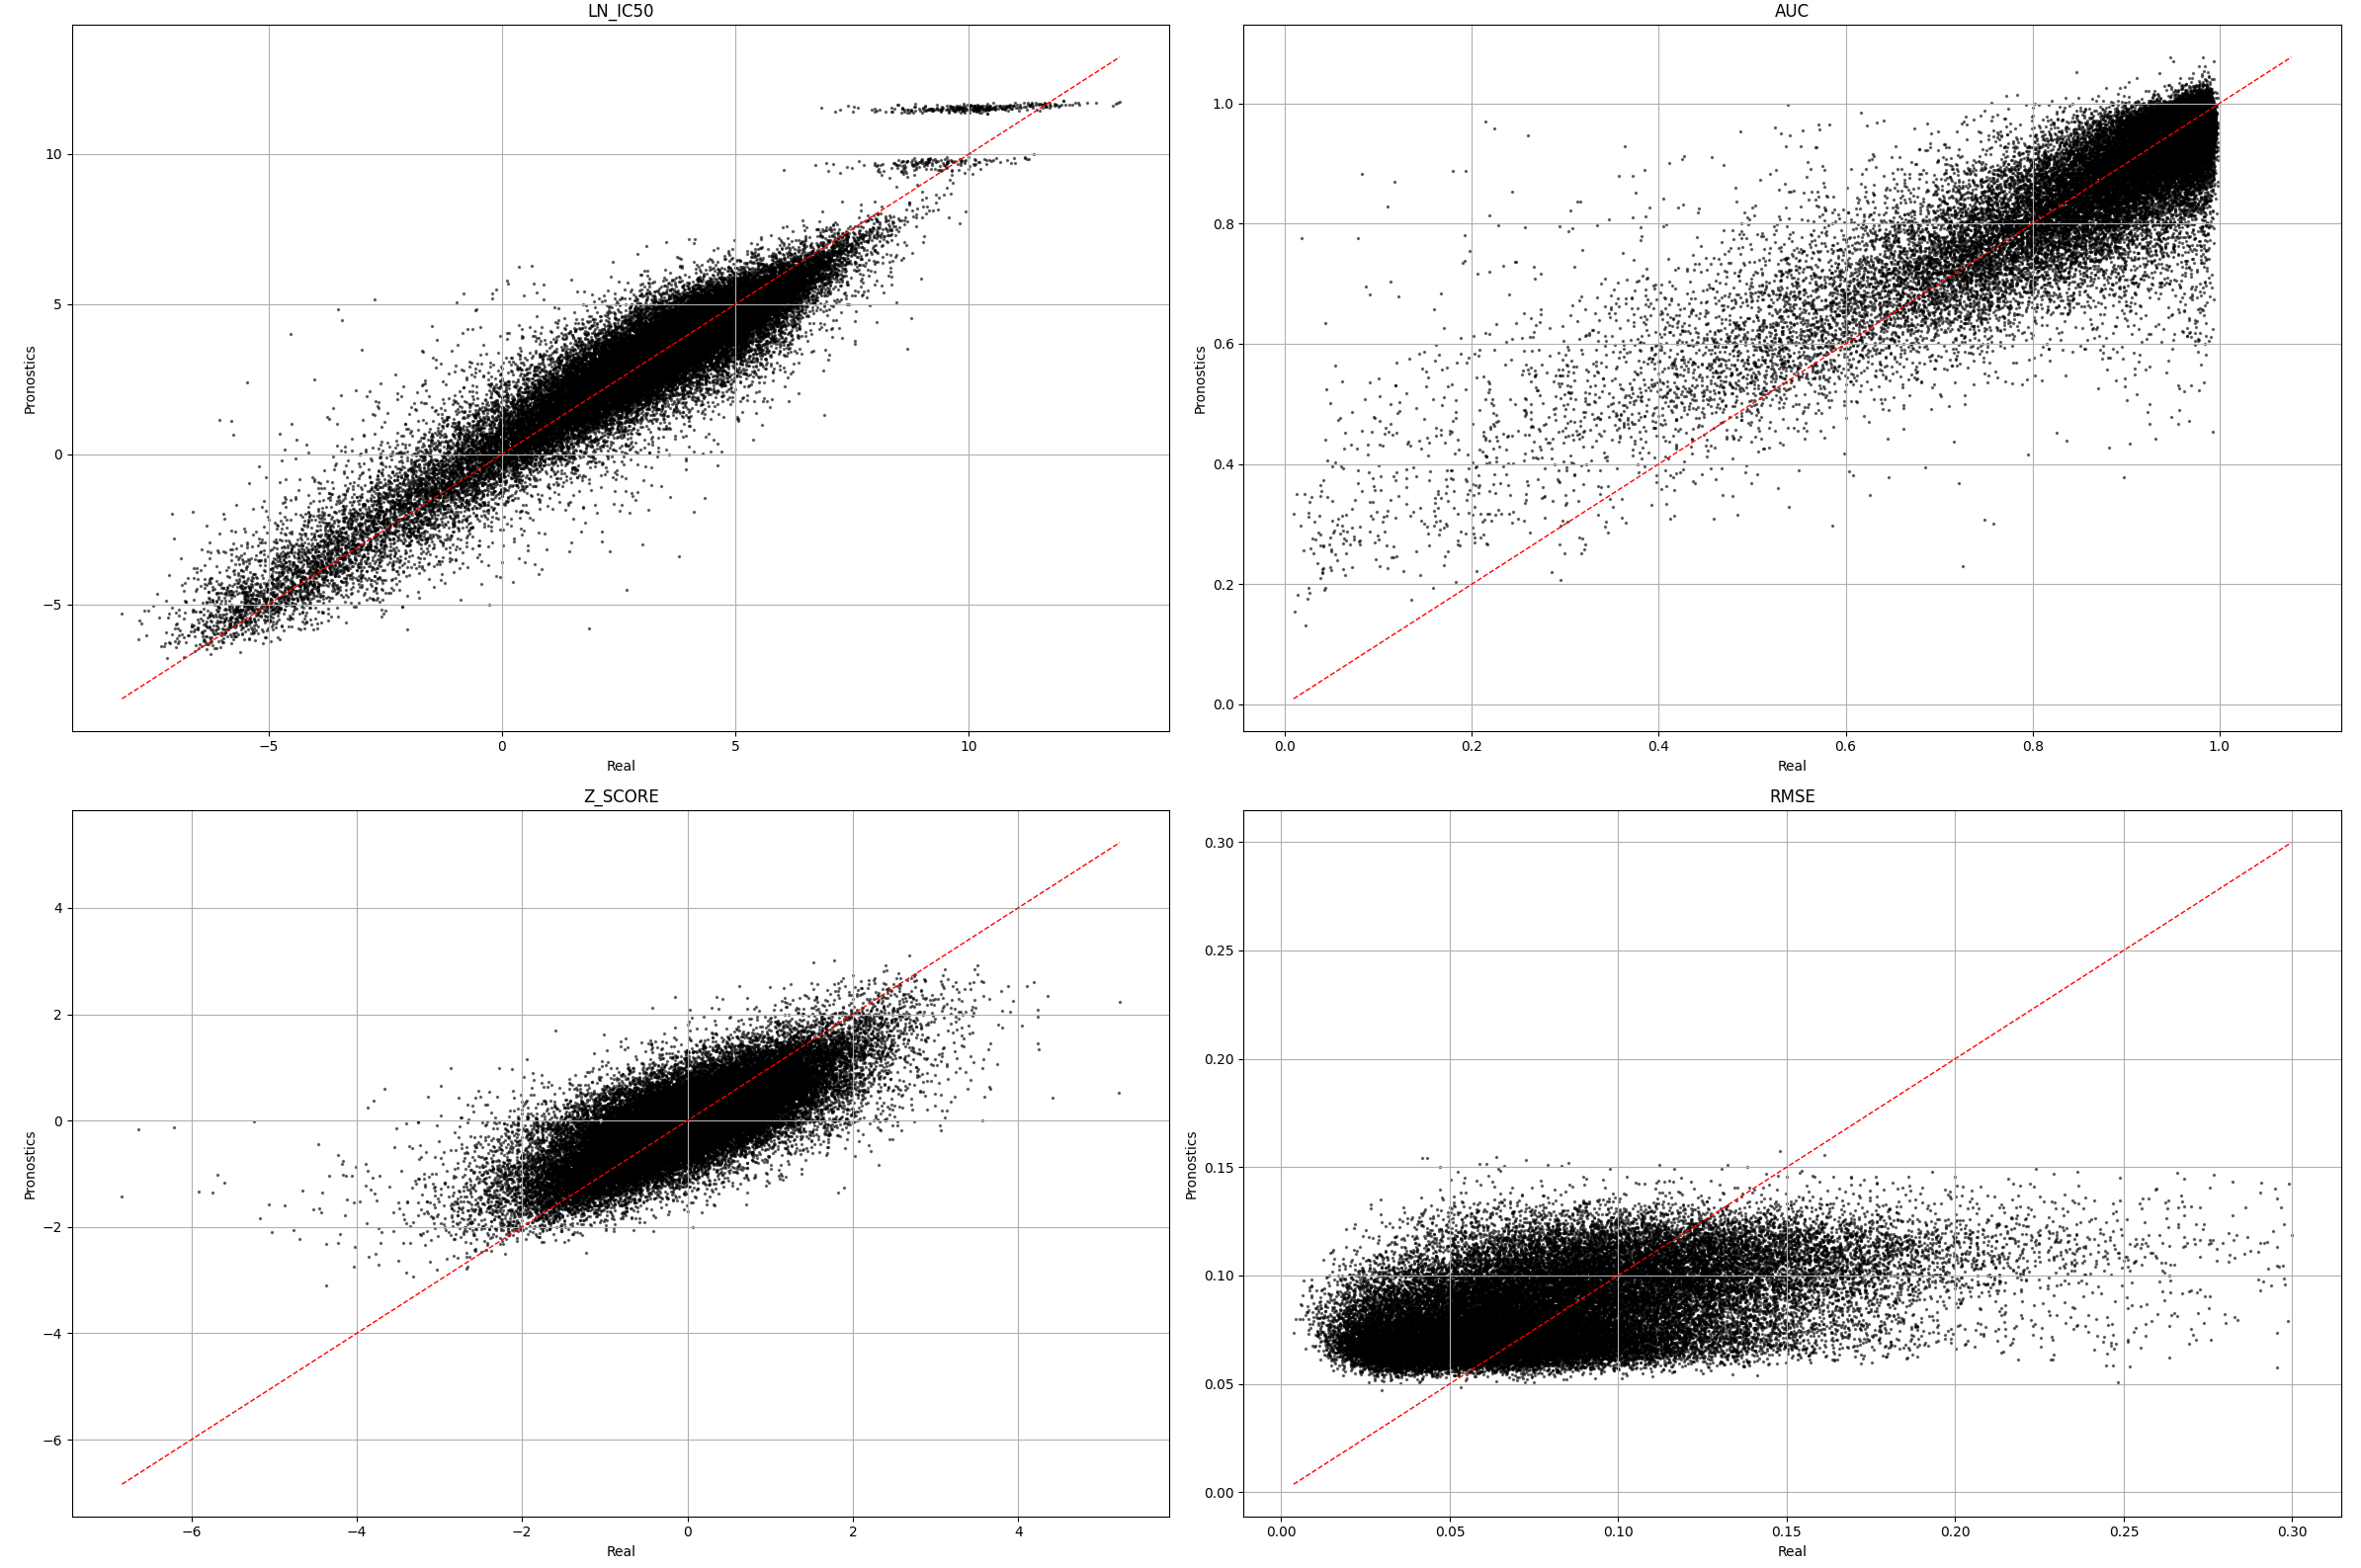
\includegraphics[width=1\textwidth]{figures/neural_net_regression_addition/output_neural_net_addition_balanced.png}
    \caption{Result of employing a neural network using convolutional layers and addition as a bridge, increasing the regularization and using SiLU as activation function.}
    \label{fig:result_addtion_reg_balanced}
\end{figure}

After this improvement in training stage, another challenge was found. The error was increased, as can be seen in Figure~\ref{fig:result_addtion_reg_balanced}. Not only did the spread for the predictions for the \(LN\_IC_{50}\) variable become wider, but the model also performed worse when predicting high values in comparation with the previous version.

This prompted a new line of research focused on improving the prediction results, trying to avoid increase the gap between training and validation again. In this situation, the best alternative was to investigate how to improve an architecture based on convolutions for other types of problems, in particular those related to images, since this is where most research has been done. 

\subsubsection{Custom architecture}

After extensive research, it became clear that one way to cancel out neurons or drastically reduce their impact was through multiplication \cite{contextgatedconvolution, gatedscnngatedshapecnns}. Thus, thinking about how to adapt this mechanism to the current architecture came to the fore, as it could be the answer to the problem. If possible, the model could learn to discriminate between points that are of no interest, providing better results.

Motivated by this idea, various ways of modifying the architecture to introduce multiplication were considered, two of which stood out:

\begin{itemize}
    \item Perform the addition as planned in the original model  and then apply the multiplication. This adaptation caused problems in the performance of the model.
    \item Replace the addition with multiplication, thereby reducing the freedom of the model compared to the previous approach. This design acts as an attention-like filter, helping the model distinguish important from irrelevant patterns. 
\end{itemize}


After observing the results of both proof-of-concept tests, the decision was clear. The implementation focused on replacing one operation with the other. As a result of this modification, the model provides better results in the test set, as evidenced by the metrics presented in Table~\ref{tab:metrics_multiplicative_gating}. Additionally, Figure~\ref{fig:result_multiply_reg_balanced} shows predictions with a lower degree of dispersion than any previous representation. This marks a key a milestone in the research, since the model achieved at this point is capable of estimating the value of the \(LN\_IC_{50}\) variable with great precision. Notably, it maintains its performance even for data points with exceptionally high \(LN\_IC_{50}\) values, not as it happened in Figure~\ref{fig:result_addtion_reg_balanced}. 

Given the absence of significant discrepancies between validation and test errors during training, this model is a strong candidate for applying explainability techniques. The insights derived could offer meaningful contributions to oncological research aimed at advancing cancer treatment

\begin{table}[H]
    \centering
    \begin{tabular}{|c|c|}
    \hline
    \textbf{Metric} & \textbf{Value} \\
    \hline
    MSE & 0.240 \\
    RMSE & 0.490 \\
    MAE & 0.242 \\
    R\textsuperscript{2} & 0.694 \\
    \hline
    \end{tabular}
    \caption{Performance metrics on the test set after incorporating the multiplicative gating mechanism.}
    \label{tab:metrics_multiplicative_gating}
\end{table}

\begin{figure}[H]
    \centering
    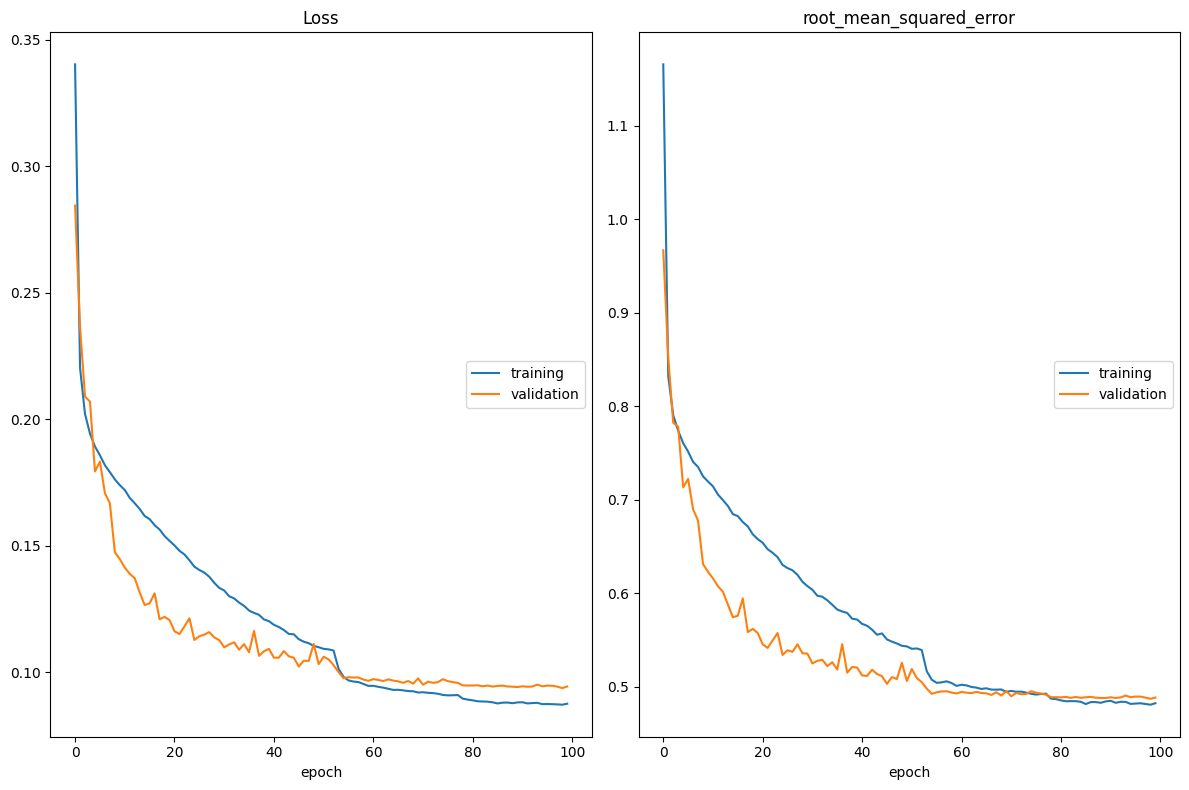
\includegraphics[width=1\textwidth]{figures/neural_net_regression_multiplication/train_logcosh_multiplication_silu.png}
    \caption{Training a neural network using convolutional layers and multiplication as a bridge.}
    \label{fig:train_multiply_reg_balanced}
\end{figure}

\begin{figure}[H]
    \centering
    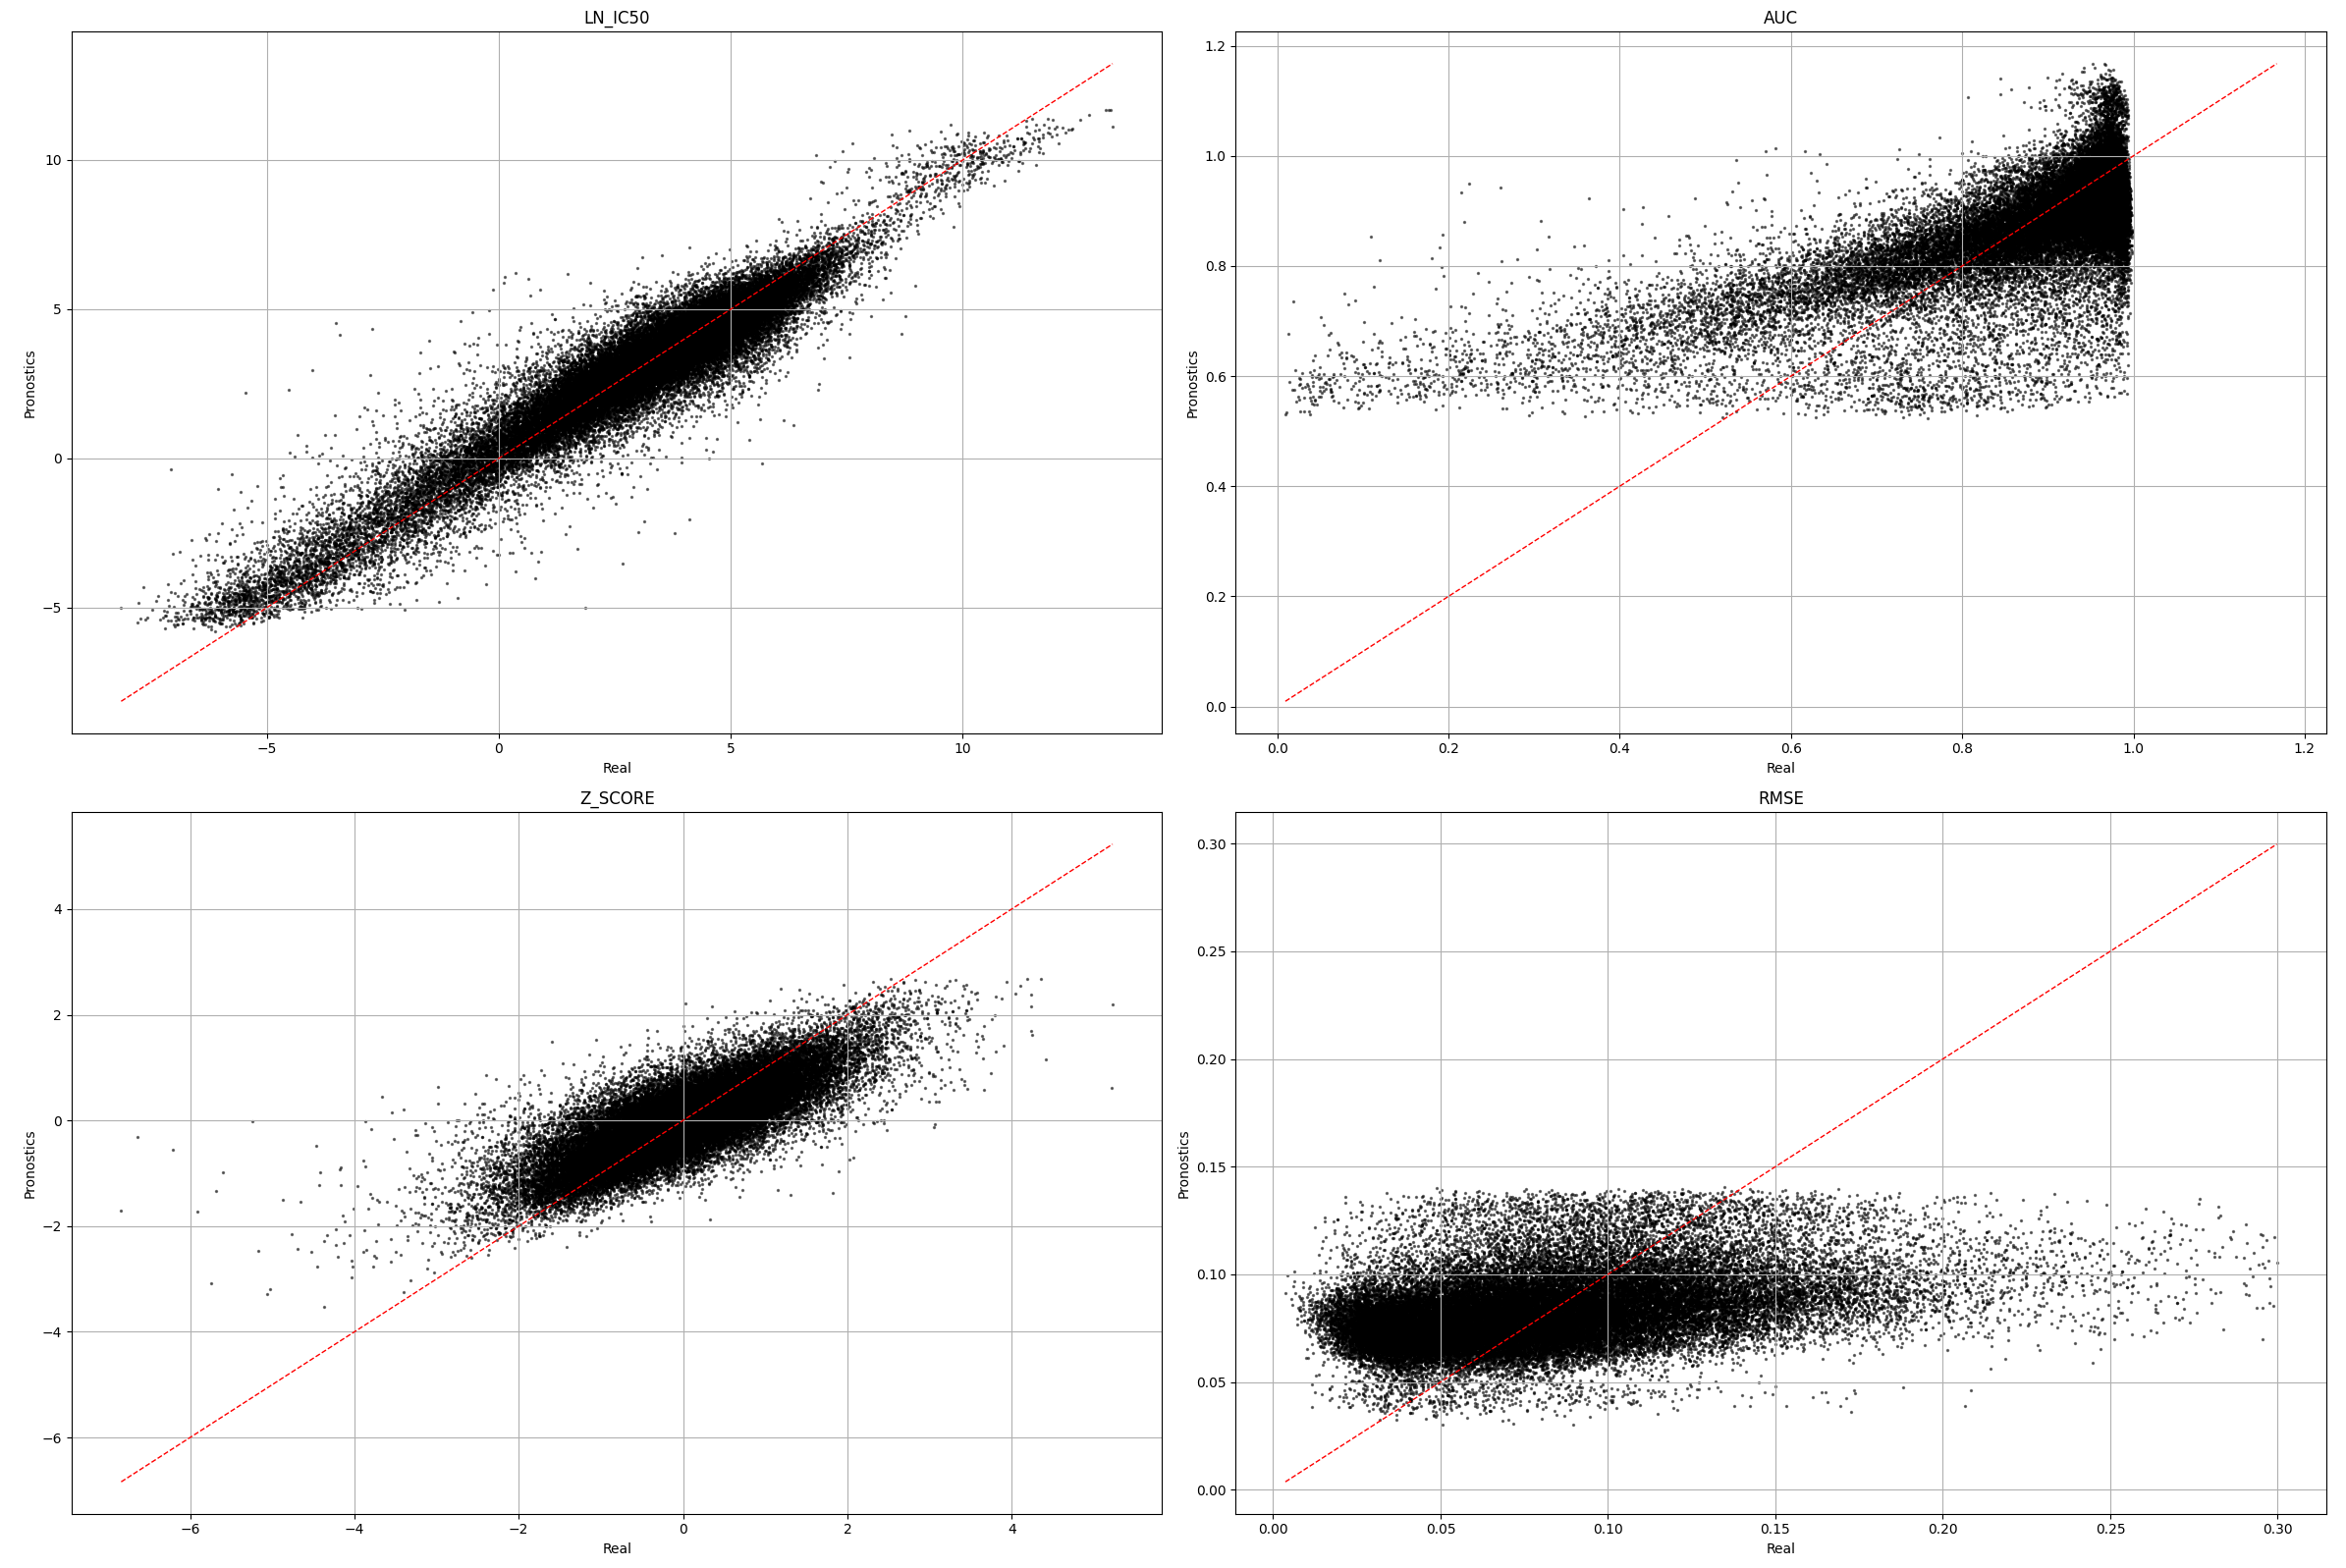
\includegraphics[width=1\textwidth]{figures/neural_net_regression_multiplication/output_neural_net_multiplication_silu.png}
    \caption{Result of employing a neural network using convolutional layers and multiplication as a bridge.}
    \label{fig:result_multiply_reg_balanced}
\end{figure}


\subsection{Application of XGBoost Regression Trees to our problem}

Currently, much of the research being conducted uses neural networks, but one should never assume that one type of architecture is always optimal for all cases. For this reason, this study includes some experiments with tree-based algorithms as well, in order to increase the knowledge of the problem. As stated at the beginning of this chapter, the chosen algorithm is XGBoost because it has shown very good results in several articles \cite{zheng2024advancedpaymentsecuritysystemxgboost, Computer-aided-boosting}.

Tree-based models have a major disadvantage compared to networks, they are typically poor at extrapolation, meaning they struggle to predict values outside the range observed during training. But even so, they are characterised by their great robustness and, due to their nature, they allow the elimination of variables without adding cost, since it is the algorithm itself that determines the features that are relevant to achieve the objective.

To enable a fair comparison between models, an XGBoost model was trained using the same dataset that was previously used for the neural networks. This approach ensures that both models are evaluated under identical conditions, allowing us to assess their respective performance accurately.

Several training sessions were performed using the XGBoost library available for Python, through which the following results were obtained:

\begin{table}[H]
    \centering
    \begin{tabular}{|c|c|}
    \hline
    \textbf{Metric} & \textbf{Value} \\
    \hline
    MSE & 1.253 \\
    RMSE & 1.119 \\
    R\textsuperscript{2} & 0.842 \\
    \hline
    \end{tabular}
    \caption{Performance metrics of the evaluated model on test set using XGBoost.}
    \label{tab:model_performance_xgboost}
\end{table}

\begin{figure}[H]
    \centering
    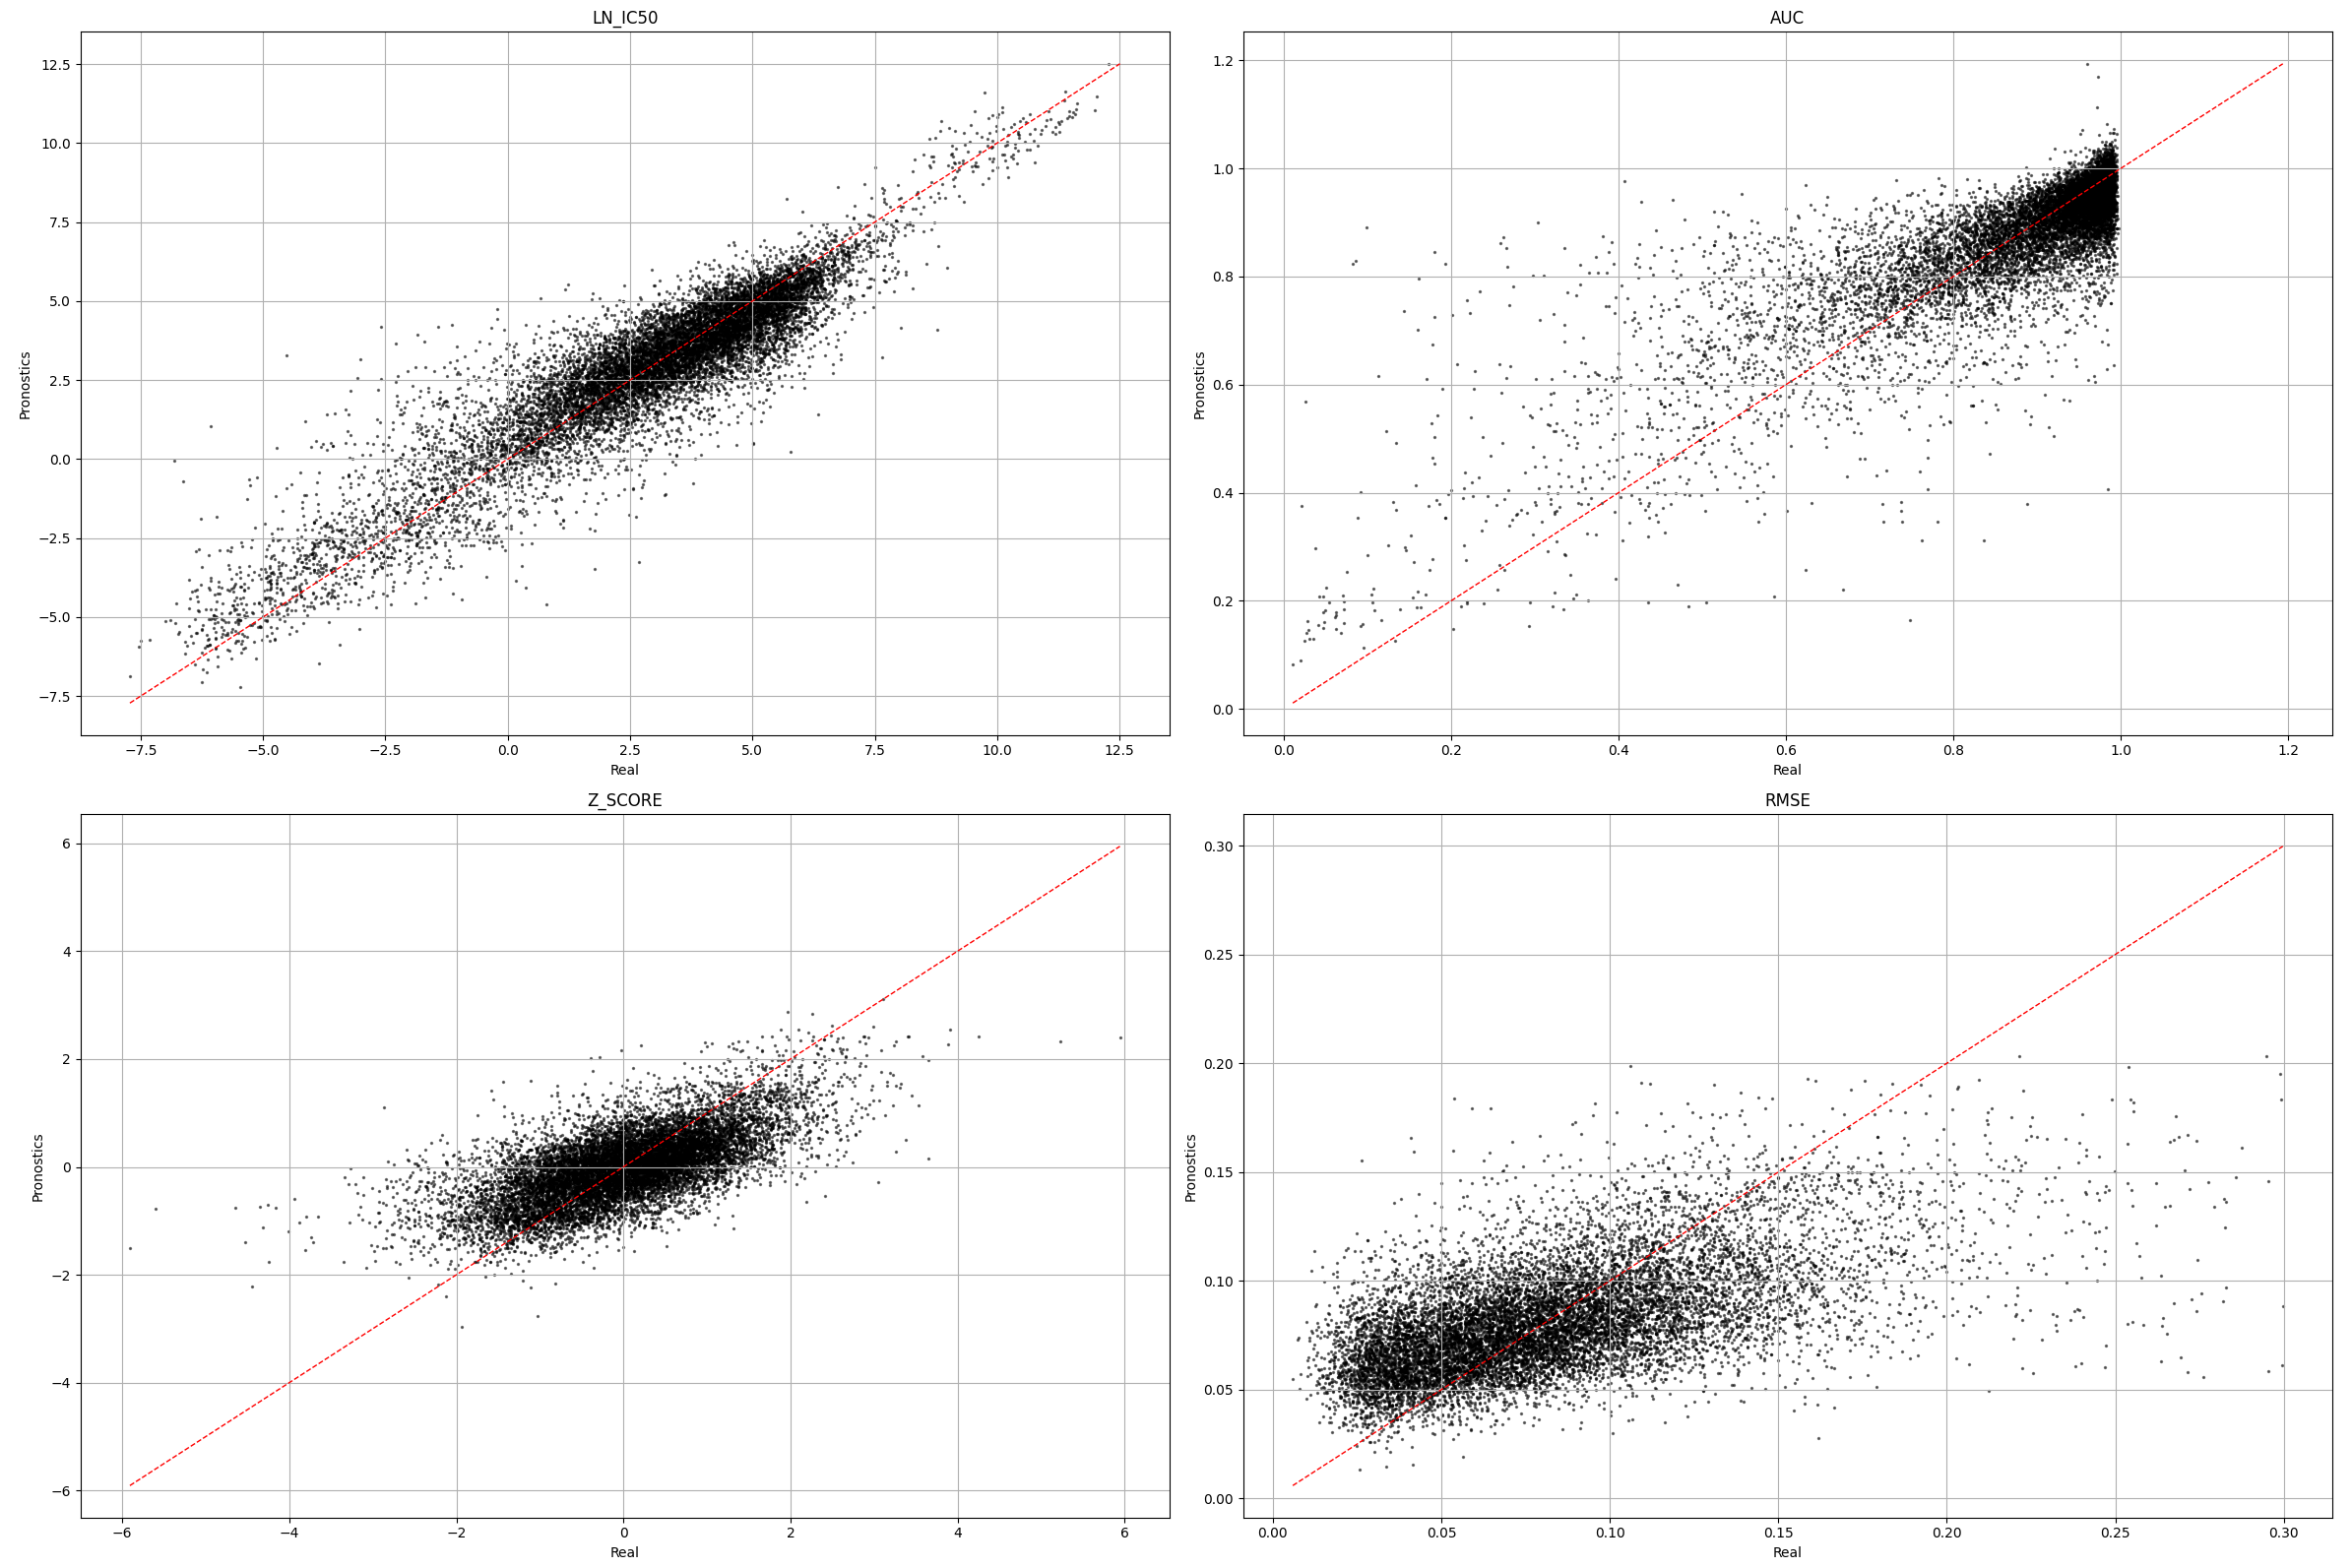
\includegraphics[width=1\textwidth]{figures/xgboost_reg/xgboost_reg_all_one_hot.png}
    \caption{Results of XGBoost with target variables encoded using one-hot.}
    \label{fig:train_xgboost_reg}
\end{figure}

Examining the performance of the model trained with XGBoost, as shown in Figure~\ref{fig:train_xgboost_reg} and Table~\ref{tab:model_performance_xgboost}, a decline in accuracy is observed compared to the neural network-based models. Specifically, the results suggest that XGBoost yields poorer predictions for the \(LN\_IC_{50}\) variable, while slightly improving the error for the remaining target variables. In other words, it increases the error in \(LN\_IC_{50}\) while reducing it for the others. However, this behavior is not desirable, as \(LN\_IC_{50}\) is the primary variable of interest. The other target variables serve merely as auxiliary signals to support the model during training and help improve its performance on the main target.

To improve the results, several hyperparameter optimization algorithms were applied, including GridSearch \cite{scikit-learn-gridsearchcv} and RandomSearch \cite{scikit-learn-randomizedsearchcv}. However, due to the presence of numerous features encoded using one-hot encoding, executing these processes required substantial computational resources, particularly in terms of RAM. This limitation posed a challenge, as such resources were not readily available. Various alternatives were evaluated to address this issue. Ultimately, ordinal encoding \cite{scikit-learn-onehotencoder} was applied to the one-hot encoded variables. This approach significantly reduced the number of columns, enabling the execution of different methods aimed at identifying dispensable variables. Among the algorithms used for this purpose were RFE \cite{scikit-learn-rfe} and SelectFromModel \cite{scikit-learn-selectfrommodel}.

In order to narrow down the variables to be eliminated, both feature selection methods, SelectFromModel and RFE, were run and those that were common to the two subsets generated were chosen. In this way, it was possible to reduce the number of variables to only 8, from 20 that were initially generated. Subsequently, RandomSearch was applied to try to find a good combination of hyperparameters, which one can be seen in Table~\ref{tab:gbm_params}. 

After that, the model was trained again. Two training were executed, the fir, using the variables with the ordinal encoder, and the second training with one-hot coding. Unfortunately, both results were of lower quality than those offered by the neural networks, as can be seen in Table~\ref{tab:xgboost_metrics_reducted}, which shows an increase in error. The best-performing model among the tested configurations was the one using one-hot encoding. It achieved the following evaluation metrics:

\begin{table}[H]
    \centering
    \begin{tabular}{|c|c|}
    \hline
    \textbf{Metric} & \textbf{Value} \\
    \hline
    MSE & 1.318 \\
    RMSE & 1.148 \\
    MAE & 0.855 \\
    R\textsuperscript{2} & 0.827 \\
    \hline
    \end{tabular}
    \caption{Performance metrics of the XGBoost model using one-hot encoding after hyperparameter optimization and variable selection.}
    \label{tab:xgboost_metrics_reducted}
\end{table}

\begin{figure}[H]
    \centering
    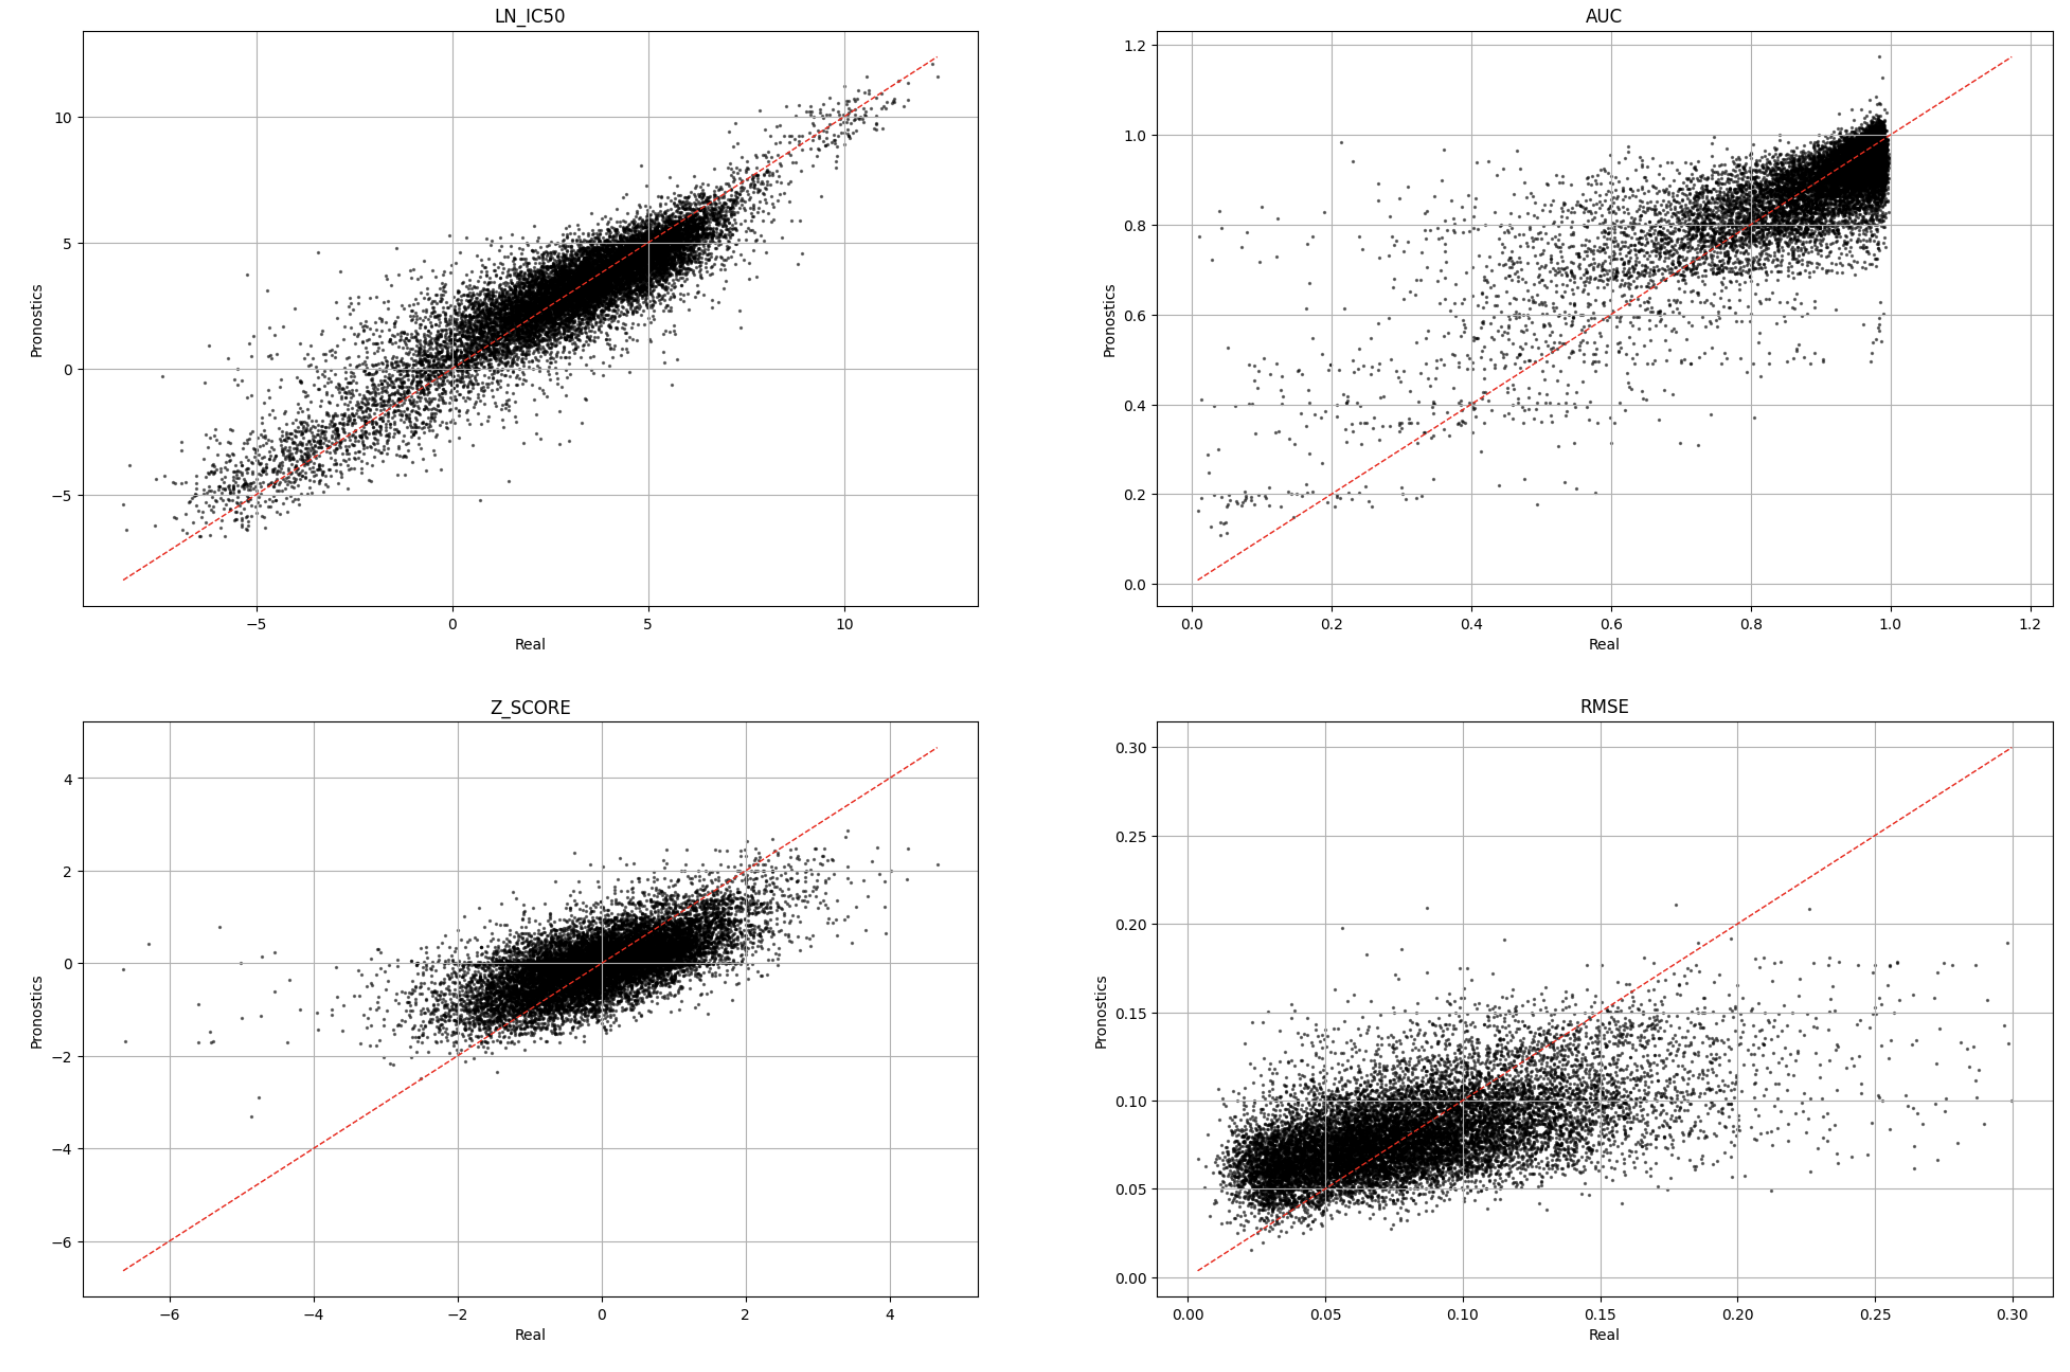
\includegraphics[width=1\textwidth]{figures/xgboost_reg/xgboost_optimized_reduced.png}
    \caption{Representation of predictions using XGBoost, together with feature reduction and hyperparameter optimisation.}
    \label{fig:xgboost_opt_red}
\end{figure}

\begin{table}[H]
    \centering
    \begin{tabular}{|c|c|}
    \hline
    \textbf{Parameter} & \textbf{Value} \\
    \hline
    \texttt{n\_estimators} & 869 \\
    \texttt{seed} & 123 \\
    \texttt{learning\_rate} & 0.028 \\
    \texttt{max\_depth} & 7 \\
    \texttt{reg\_alpha} & 0.040 \\
    \texttt{reg\_lambda} & 0.492 \\
    \texttt{max\_leaves} & 328 \\
    \hline
    \end{tabular}
    \caption{Hyperparameters of the gradient boosting model after applying hyperparameter optimization.}
    \label{tab:gbm_params}
\end{table}

\section{A classification problem}

The previous section has focused on continuous target variables, except for Drug Response, successfully developing a neural network-based regressor capable of predicting the \(LN\_IC_{50}\) variable with high accuracy, achieving an RMSE below 0.5. Building upon this strong foundation, the next step aims to bring the model closer to a real-world clinical application. To do this, the continuous \(LN\_IC_{50}\) variable is discretised into 25 equally spaced intervals, offering a practical approximation of dosage levels. 

This number of intervals has not been selected at random, but rather as a result of analysing the growth of entropy as a function of the number of divisions, particularly by observing the slope of this evolution. Maximising entropy allows to obtain a highly representative set, but an excessive number of divisions can introduce noise or redundancy. To avoid this problem, the slope of the entropy curve is analysed in order to identify an inflection point that indicates a balance between representativeness and stability. Thus, Figure~\ref{fig:intervalEntropy} illustrates the evolution of both entropy and the slope of its evolution. Based on this information, a division of 25 intervals is proposed, as this represents a midpoint between the slope and the increase in entropy. To carry out these operations, the code shown in Listing~\ref{cod:intervalEntropy} has been used.

\begin{figure}[H]
    \centering
    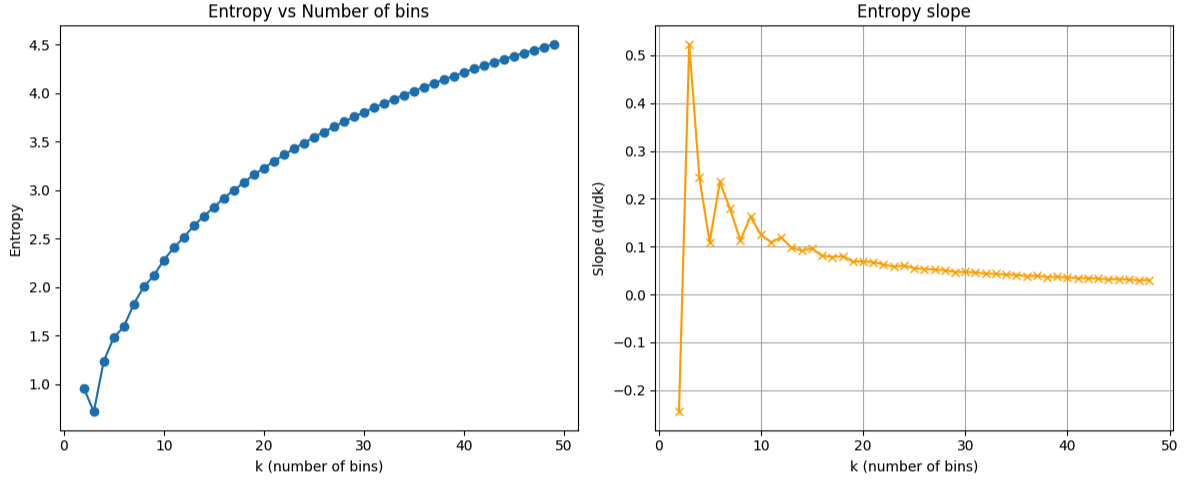
\includegraphics[width=1\textwidth]{figures/intervalEntropy.png}
    \caption{Representation of entropy evolution based on the number of bins.}
    \label{fig:intervalEntropy}
\end{figure}

The range in which the value of \(LN\_IC_{50}\) is found must be understood as the number of pills the patient should take. This idea makes a lot of sense, as getting closer to the concept of prescribing a certain number of pills allows to be somewhat more lax with the error made. For example, if two ibuprofens are taken instead of one, the negative effect is not appreciable. However, this is not the case when six are taken instead of one. Therefore, it can be inferred that making a slight error is not as serious as making a large one, an aspect that should certainly be considered when calculating the error.

Before any model is trained, the data will be visualized graphically to assess their separability, specifically, to determine whether the class ranges overlap in feature space or not. Since the dataset, after applying the ordinal encoder, contains more than 20 variables, direct representation is not feasible. Therefore, a dimensionality reduction process will be performed to project the data into 2D and 3D spaces, allowing for easier interpretation.

First, t-SNE \cite{cai2022theoreticalfoundationstsnevisualizing} will be used to perform the compression process. This algorithm is highly effective at capturing local relationships; that is, within a group, the relationships between data points can be accurately preserved. This will allow an assessment of whether points belonging to the same group are located close together in space. If they are not, it indicates higher data variance, which would make it more challenging for a model to correctly predict group membership.

For this purpose, the t-SNE method from scikit-learn \cite{scikit-learn-tsne} will be used. However, the algorithm is computationally expensive. To accelerate execution, the data obtained from the initial run will be saved using NumPy, so that subsequent executions can bypass the computational step. This process is illustrated in Listing~\ref{cod:tsne}.

\begin{figure}[H]
    \centering
    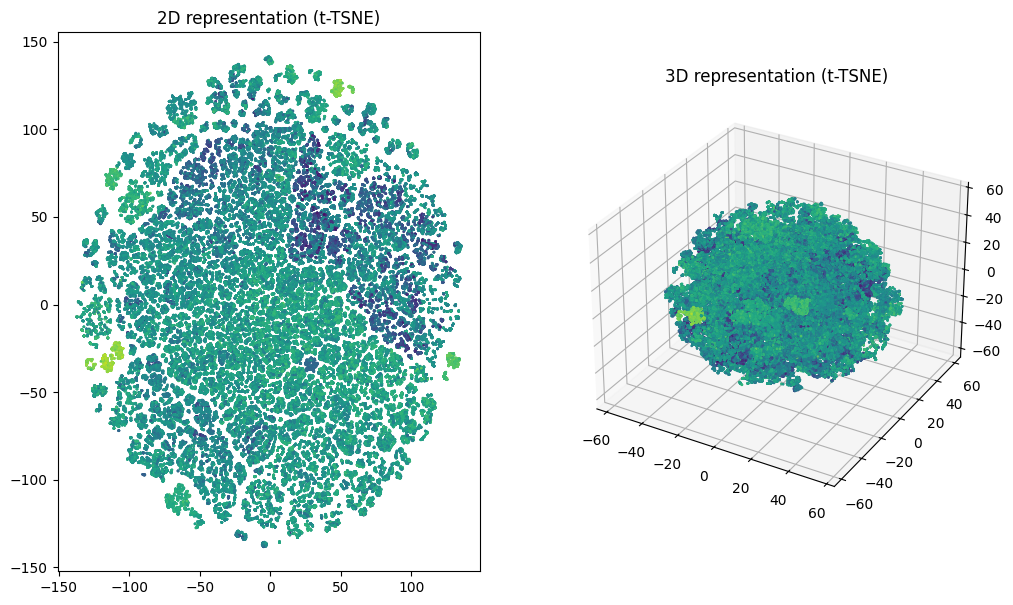
\includegraphics[width=1\textwidth]{figures/data_representation/tsne.png}
    \caption{Representation of the data by t-SNE, where it can be seen the separation between points of the same cluster.}
    \label{fig:tsne}
\end{figure}

As a result, the representation shown in Figure~\ref{fig:tsne} is obtained, in which the groups appear to be clearly distinguishable. However, a new question arises: although the clusters seem to be located close to one another in the plot, it is not certain whether this proximity reflects the true structure of the data, since t-SNE does not accurately capture global relationships, that is, the relationships between different groups.

To address this, UMAP \cite{mcinnes2020umapuniformmanifoldapproximation} will be used, as it is capable of preserving both local and global non-linear relationships. The implementation will be carried out using the umap-learn library \cite{umap-docs}, as demonstrated in Listing~\ref{cod:umap}. Similar to t-SNE, UMAP is computationally expensive; therefore, the same data-saving strategy will be applied to avoid repeated computations in future executions.

As a result, it can be observed in Figure~\ref{fig:umap} that the clusters are indeed well separated. Therefore, it can be assumed a priori that applying predictive models may yield good results.

\begin{figure}[H]
    \centering
    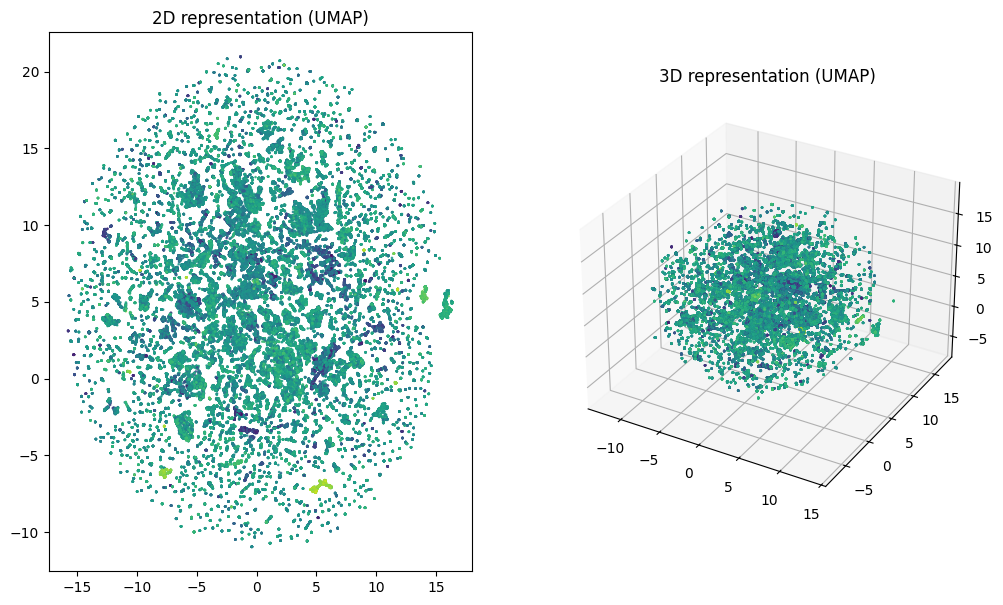
\includegraphics[width=1\textwidth]{figures/data_representation/umap.png}
    \caption{Representation of the data by UMAP, where it can be checked the distance between the different groups and their internal elements.}
    \label{fig:umap}
\end{figure}


\section{Discovering the correct group using Neural Networks}

The objective of this section is to estimate the number of doses required by a patient using a neural network. To accomplish this, the previously developed architecture must be adapted to effectively model the problem, beginning with the dataset that includes a discretized version of the target variable.

The process has been divided into three main stages:

\begin{enumerate}
    \item Adaptation of the existing architecture.
    \item Expansion paths
    \item Refinement of the loss function.
\end{enumerate}

\subsubsection{Adaptation of the existing architecture}

Building on the previously trained neural network model, the objective of this section is to obtain a new network capable of estimating the number of doses of a drug needed to treat a person. 
Acquiring a certain degree of intuition about how current architecture deals with classification issues is crucial to making changes that truly add value. Therefore, initially the changes will be subtle, i.e., only very specific sections of the architecture will be modified. In this way, after each modification that leads to an improvement in performance, it will be translated into the new goal to be achieved. To achieve this, it is necessary to modify both the loss function and the output layer of the model to make the predictions compatible with the classification.

Thus, the error function was replaced by categorical cross-entropy, which is one of the most used, with the aim of testing the model's accuracy. With regard to the model output, Softmax is the most recommended for this type of classification problem, as it provides a probability for each possible class. 

As there is more than one target variable, the network must have more than one output layer simultaneously, as can be seen in Listing~\ref{cod:class_net_v1}.

Once model training began, it successfully completed 100 epochs. The learning curves, shown in Figure~\ref{fig:train_class_net_v1}, reveal that the model achieves better performance on the validation set than on the training set, an uncommon but noteworthy behavior. However, despite this apparent advantage, the overall quality of the predictions remains limited, with accuracy values not exceeding 0.35, as can be seen in Table~\ref{tab:best_val_ln_ic50_metrics_net_class_v1}. This indicates that, although generalization may be occurring, the model still struggles to produce reliable predictions. Furthermore, depending on the progress of the training, the model would be able to improve if the number of available epochs were increased.

\begin{figure}[H]
    \centering
    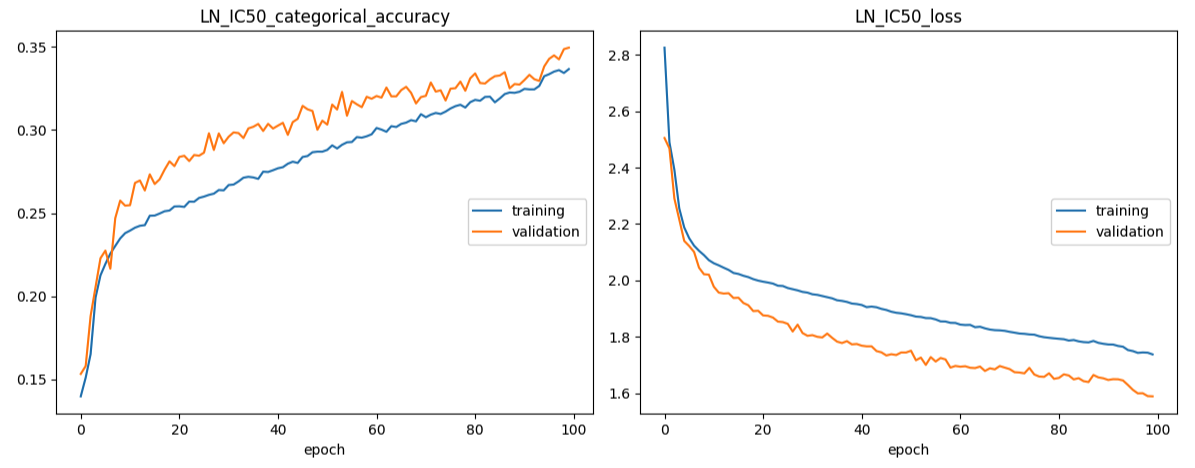
\includegraphics[width=1\textwidth]{figures/neural_net_classification/classification_mse_v1.png}
    \caption{Progress of model training after replacing the error function with cross-entropy and the output layer with a multi-class layer with softmax activation function. Better performance is observed in the validation set compared to the training set.}
    \label{fig:train_class_net_v1}
\end{figure}

\begin{table}[H]
    \centering
    \begin{tabular}{|l|c|}
    \hline
    \textbf{Validation Metric} & \textbf{Best Value} \\
    \hline
    LN\_IC50\_Categorical\_Accuracy & 0.349 \\
    LN\_IC50\_Loss & 2.505 \\
    \hline
    \end{tabular}
    \caption{Best validation results for LN\_IC50 metrics.}
    \label{tab:best_val_ln_ic50_metrics_net_class_v1}
\end{table}

\subsubsection{Expansion paths}

Refining the architecture so that the model is able to correctly capture the patterns present in the dataset is the next step towards achieving better results. Thus, the architecture currently proposed to act as a classifier has one main weakness: the error function. This is because it is unable to adjust to unbalanced data, for this reason it will be replaced by categorical focal cross-entropy. Depending on which one yields the most promising results, one or the other will be selected to form part of a customised function that takes into account the importance of large errors.

Additionally, giving greater relevance to the \(LN\_IC_{50}\) variable will help the model focus its efforts on correctly predicting this output. Without neglecting the extra knowledge provided by the others, thus serving as a support.

\subsubsection{Expansion paths: Loss function}

Among the loss functions suitable for classification tasks involving imbalanced classes, categorical focal cross-entropy is particularly worth considering. As an extension of the standard categorical cross-entropy, it introduces mechanisms specifically designed to mitigate the effects of class imbalance by emphasizing harder-to-classify examples. Applying this loss function can offer a useful indication of whether the class imbalance is significantly influencing model performance. 

The formula of this function is:

\[
\text{FL}(y, \hat{y}) = -\sum_{i=1}^{C} \alpha_i \, y_i \, (1 - \hat{y}_i)^\gamma \log(\hat{y}_i)
\]

\begin{itemize}
    \item \( C \): Total number of classes.
    \item \( y_i \): True label for class \( i \) (one-hot encoded).
    \item \( \hat{y}_i \): Predicted probability for class \( i \).
    \item \( \alpha_i \): Class weight (optional, used for class balancing).
    \item \( \gamma \): Focusing parameter (typically set to 2).
    \item \( (1 - \hat{y}_i)^\gamma \): Modulating factor that down-weights easy (high-confidence) examples.
\end{itemize}

Since the implementation is being carried out using the Tensorflow API, making this change is very simple. It only requires changing one line of text, as can be seen in Listing~\ref{cod:class_net_v2}.

\begin{figure}[H]
    \centering
    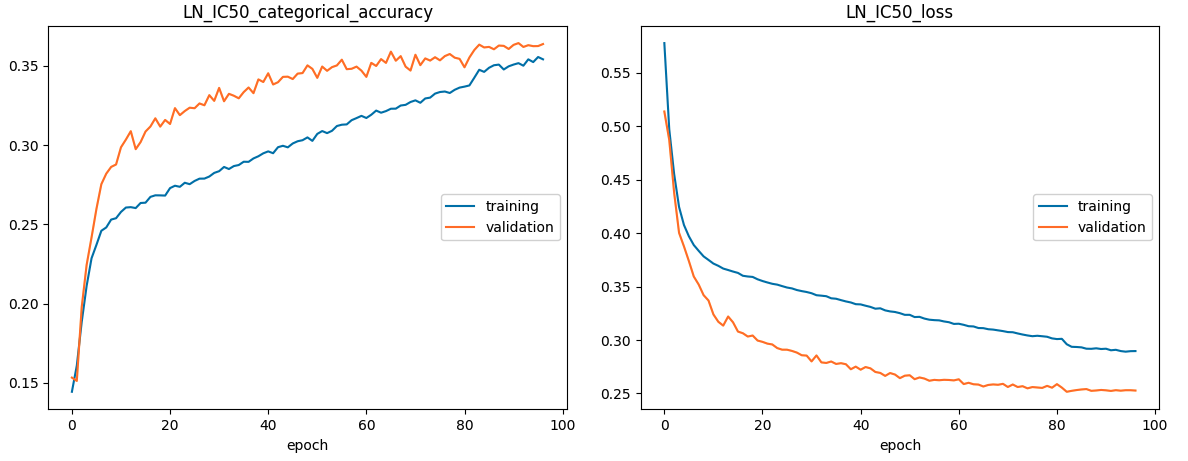
\includegraphics[width=1\textwidth]{figures/neural_net_classification/classification_mse_v2.png}
    \caption{Model training progress applying categorical focal loss.}
    \label{fig:train_class_net_v2}
\end{figure}

\begin{table}[H]
    \centering
    \begin{tabular}{|l|c|}
    \hline
    \textbf{Validation Metric} & \textbf{Best Value} \\
    \hline
    LN\_IC50\_Categorical\_Accuracy & 0.383 \\
    LN\_IC50\_Loss & 0.504 \\
    \hline
    \end{tabular}
    \caption{Best validation results for LN\_IC50 metrics using focal loss.}
    \label{tab:best_val_ln_ic50_focal}
\end{table}

The results obtained after this new modification are extremely interesting. Both models, the previous one and this one, perform better on the validation set than on the training set. However, in this case, it can be seen that it was necessary to reduce the learning rate halfway through training in order to continue improving. In the previous case, the learning rate did not need to be reduced to obtain a substantial improvement in performance, as illustrated in Figure~\ref{fig:train_class_net_v1}. 

In this second training session, although better results are obtained than in the previous one, as shown in Table~\ref{tab:best_val_ln_ic50_focal}, the model's progression is less promising, as can be seen in igure~\ref{fig:train_class_net_v2}.

This can lead to two main ideas:

\begin{itemize}
    \item The dataset contains some unbalanced classes. Therefore, in order to learn how to classify them correctly, the first model must invest more time, while the second, thanks to the focal error function, is able to learn faster. However, this second model reaches a plateau even after reducing the learning rate.
    \item Although the model that uses categorical error learns more slowly, it seems to have more potential for improvement, since in the case of the model that incorporates focal loss, the performance slope is less pronounced.
\end{itemize}

\subsubsection{Expansion paths: Priorities}

Due to the high number of outputs in the current architecture, the model may attempt to learn all targets with equal emphasis, or worse, prioritize outputs that are not related to \(LN\_IC_{50}\). To address this, a weighting strategy was proposed in which the importance of each output is adjusted. This aims to improve the prediction performance for \(LN\_IC_{50}\) by giving it higher priority during training.

This modification was implemented using the Keras Functional API, as shown in Listing~\ref{cod:class_net_v3}. The loss contributions from all output layers were maintained, except for the one corresponding to \(LN\_IC_{50}\), which was assigned 50\% more weight. The objective is to ensure that the model continues to consider the auxiliary outputs while explicitly encouraging better performance on the primary target, \(LN\_IC_{50}\).

Thanks to this approach, a considerable improvement was achieved during training, as shown in Figure~\ref{fig:train_class_net_v3} and Table~\ref{tab:best_val_ln_ic50_wheighting}. Here, both accuracy and error have improved. Once again, it was necessary to reduce the learning rate during training.

\begin{figure}[H]
    \centering
    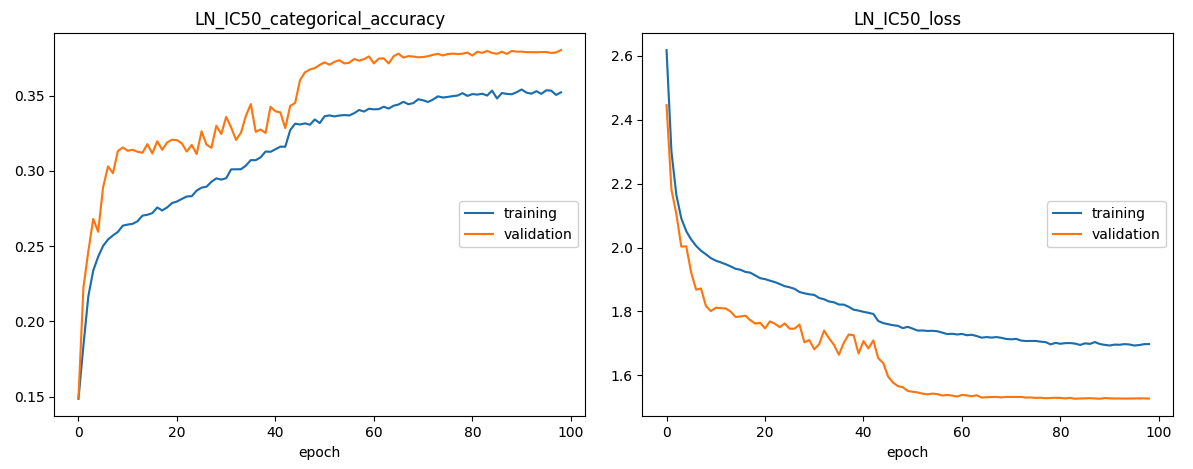
\includegraphics[width=1\textwidth]{figures/neural_net_classification/classification_mse_v3.png}
    \caption{Model training progress by changing the importance of outputs.}
    \label{fig:train_class_net_v3}
\end{figure}

\begin{table}[H]
    \centering
    \begin{tabular}{|l|c|}
    \hline
    \textbf{Validation Metric} & \textbf{Best Value} \\
    \hline
    LN\_IC50\_Categorical\_Accuracy & 0.384 \\
    LN\_IC50\_Loss & 2.496 \\
    \hline
    \end{tabular}
    \caption{Best validation results for \(LN\_IC_{50}\) metrics after applying output weighting.}
    \label{tab:best_val_ln_ic50_wheighting}
\end{table}

Everything seems to indicate that adjusting the weights of the outputs provides an increase in the model's performance. Likewise, during this training, it can be observed how, once again, the categorical cross-entropy error function has provided the necessary dynamism to improve the quality of the predictions by reducing the learning rate in around the epoch 80.

\subsubsection{Refinement of the loss function}

The experimental results suggest that performance can be improved by carefully designing the training process, specifically through a combination of output weighting and an appropriately chosen loss function.

While selecting the optimal combination of weights often involves empirical tuning, the choice of loss function is more critical, as it must be tailored to both the characteristics of the data and the nature of the problem. It is important to recall that the objective is not merely to predict the exact number of doses, but to minimize the severity of misclassifications. For example, mispredicting by one dose is less significant than mispredicting by five. Consequently, the loss function must reflect this asymmetry in error severity.

Additionally, the loss must support effective learning; otherwise, there is a risk of stagnation during training. To address these requirements, a custom loss function was developed for the final version of the classification model, as shown in Listing~\ref{cod:class_net_v4}. This function penalizes predictions progressively based on their distance from the correct class, encouraging the model to make closer, even if not exact, predictions. As a result, the number of highly incorrect classifications is significantly reduced.

As a result of all these modifications, the model significantly increases performance and reduces the difference between training and validation, all of which can be seen in Figure~\ref{fig:train_class_net_v4}. This translates into more accurate and reliable predictions outside the training set.

\begin{figure}[H]
    \centering
    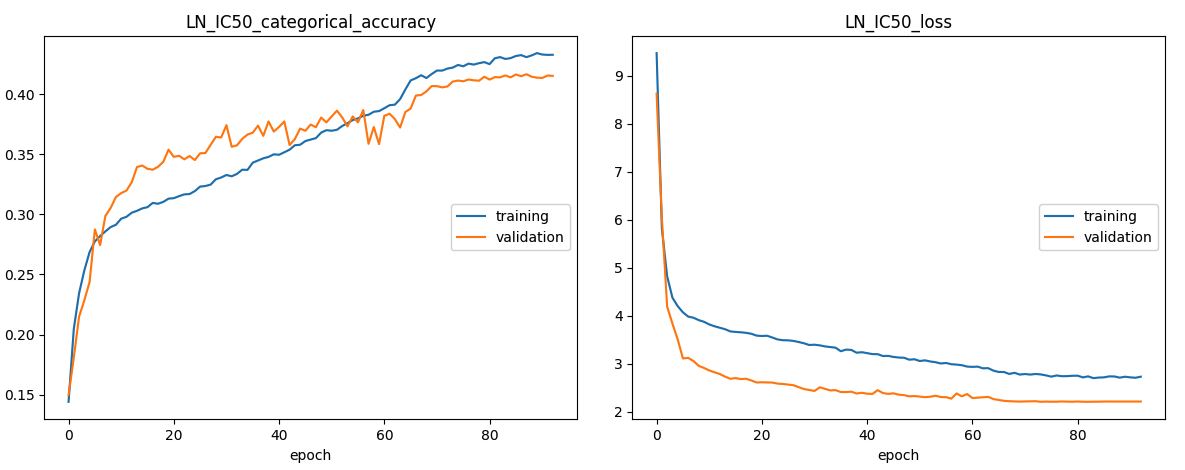
\includegraphics[width=1\textwidth]{figures/neural_net_classification/classification_custom_loss.png}
    \caption{Progress of model training applying a customised error function, which takes into account both accuracy and the difference between the actual and predicted values.}
    \label{fig:train_class_net_v4}
\end{figure}

\begin{table}[H]
    \centering
    \begin{tabular}{|l|c|}
    \hline
    \textbf{Validation Metric} & \textbf{Best Value} \\
    \hline
    LN\_IC50\_Categorical\_Accuracy & 0.412 \\
    LN\_IC50\_Loss & 2.195 \\
    \hline
    \end{tabular}
    \caption{Best validation results for LN\_IC50 metrics using the custom loss function.}
    \label{tab:best_val_ln_ic50_customloss}
\end{table}

\begin{figure}[H]
    \centering
    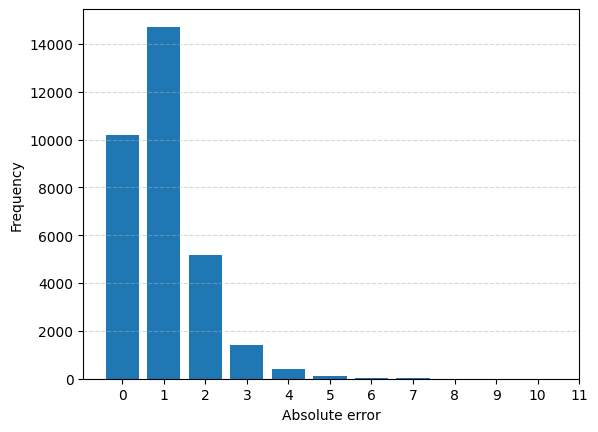
\includegraphics[width=1\textwidth]{figures/neural_net_classification/catogorical_net_barplot.png}
    \caption{Bar chart representation of the absolute error committed in the test set. It allows us to verify that the model predicts with a low degree of error.}
    \label{fig:train_class_net_v4_barplot}
\end{figure}

\begin{table}[H]
    \centering
    \begin{tabular}{|l|c|}
    \hline
    \textbf{Test Metric} & \textbf{Value} \\
    \hline
    MSE & 1.218 \\
    RMSE & 1.103 \\
    R\textsuperscript{2} & 0.878 \\
    \hline
    \end{tabular}
    \caption{Regression performance metrics on the test set for LN\_IC\_50 using a neural network with custom loss function.}
    \label{tab:test_regression_metrics:net_class_v4}
\end{table}

However, there is one aspect that cannot be assessed from the graph in Figure~\ref{fig:train_class_net_v4}. In this iteration, an error function has been defined that should prevent large discrepancies between reality and prediction. This feature is corroborated in Figure~\ref{fig:train_class_net_v4_barplot}, which illustrates a histogram in which the highest percentage of errors are between 0 and 1 doses. Therefore, the model effectively meets expectations.

Reaching this point in the research represents a milestone in the study, as the model is capable of deciding how many doses to administer, with a single-dose error in most cases. This allows for better management of prescriptions, thus improving patients' quality of life.

\section{Testing XGBoost as a classifier}

In this section, the method applied is XGBoost in a multi-class classification setting, using the discretised variable \(LN\_IC_{50}\) as in previous experiments. The aim is to evaluate its predictive power and compare it with the results obtained using deep learning approaches.

Beyond accuracy, it is particularly interesting how XGBoost handles the ordinal nature of the target variable, where misclassifying a class by 1 is much less serious than misclassifying it by 5 or more. To achieve this, evaluations will be carried out using standard metrics, such as accuracy, but also some that take into account the distance between the prediction and the actual classes, including MAE and RMSE.

As the dynamic applied throughout the research, the model will be refined as the reading progresses. First, training will be carried out where only accuracy will be taken into account, and then training will also evaluate the difference between prediction and expected class. This initial process will allow us to compare and verify that this approach is the most appropriate.

\subsubsection{Focusing on classification}

To conduct the research using xgboost and focusing solely on the accuracy of the result, the most appropriate objective function is softmax. This setting enable multi-class classification, by directly modeling the probability distribution over all classes. Otherwise, the architecture would have to be modelled as one vs rest system, which would require a binary classifier for each class. This would increase the time and effort required.

For evaluating model performance, the chosen loss function is categorical cross-entropy, referred to in the XGBoost Python library as Multi-Class Log Loss (mlogloss). This metric is particularly appropriate because it not only assesses classification correctness but also takes into account the confidence of the predicted probabilities, in this way, a more nuanced assessment is provided than simple accuracy.

The flaw in this approach is that it does not take into account the severity of major errors. In fact, Figure~\ref{fig:barplot_xgboost_v1} shows how the results obtained using this model falls significantly short of those produced by the neural network. This is further supported by the metrics shown in Table~\ref{tab:xgboost_classification_metrics_v1}, which reveal a substantial increase in error.

\begin{figure}[H]
    \centering
    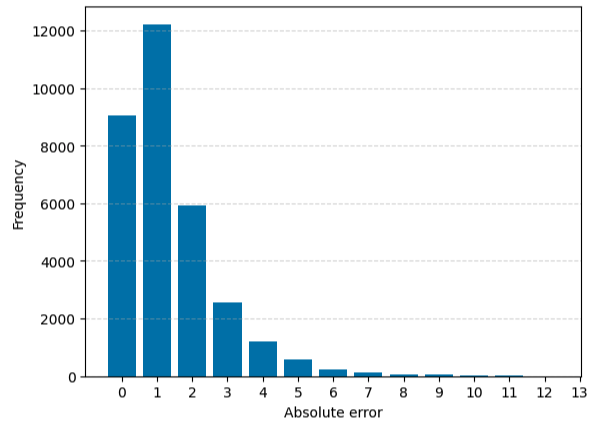
\includegraphics[width=1\textwidth]{figures/xgboost_class/xgboost_class_v1_softmax.png}
    \caption{Representation of the absolute error committed with the test set using XGBoost and softmax. A substantial increase in error is observed, with the largest error committed being 11.}
    \label{fig:barplot_xgboost_v1}
\end{figure}

\begin{table}[H]
    \centering
    \begin{tabular}{|l|c|}
    \hline
    \textbf{Test Metric} & \textbf{Value} \\
    \hline
    MSE & 2.766 \\
    RMSE & 1.663 \\
    R\textsuperscript{2} & 0.724 \\
    \hline
    \end{tabular}
    \caption{Performance metrics on the test set for \(LN\_IC_{50}\) using XGBoost classifier predictions interpreted as numerical outputs.}
    \label{tab:xgboost_classification_metrics_v1}
\end{table}

\subsubsection{Prioritizing distance to the right class}

Applying a function that shows the importance of being close to the correct class should improve the quality of the model. In the case of XGBoost, the function used is the mean square error (MSE). In addition, it is necessary to modify the evaluation metric, in this case the root mean square error (RMSE), to facilitate the interpretation of progress.

After a series of training sessions, a result similar to that of neural networks was obtained, without reaching the same quality, but improving on the previous version. This can be seen in Figure~\ref{fig:barplot_xgboost_v2}, which shows how the proportion changes, increasing the number of cases in which only one error is made, or even none at all. It also reduces all the others, as reflected in the metrics in Table~\ref{tab:xgboost_classification_metrics_v2}, where the maximun error is 12.

\begin{figure}[H]
    \centering
    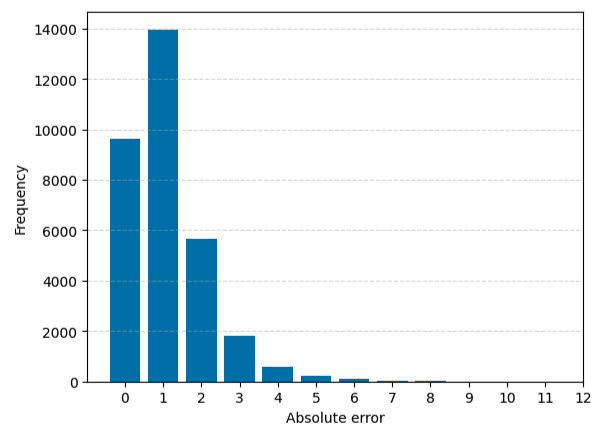
\includegraphics[width=1\textwidth]{figures/xgboost_class/xgboost_class_v2_mse.png}
    \caption{Representation of the absolute error committed with the test set using XGboost and MSE. A substantial increase in error is observed, with the largest error committed being 12.}
    \label{fig:barplot_xgboost_v2}
\end{figure}

\begin{table}[H]
    \centering
    \begin{tabular}{|l|c|}
    \hline
    \textbf{Test Metric} & \textbf{Value} \\
    \hline
    MSE & 2.381 \\
    RMSE & 1.543 \\
    R\textsuperscript{2} & 0.834 \\
    \hline
    \end{tabular}
    \caption{Performance metrics on the test set using XGBoost with \texttt{reg:squarederror}.}
    \label{tab:xgboost_classification_metrics_v2}
\end{table}

By applying the same distance-aware approach used in neural networks to the XGBoost model, the result obtained is very similar. Two key aspects of this result must be taken into account:

\begin{itemize}
    \item Accuracy of predictions: While the overall performance is similar in terms of trend, the quality of the model is slightly lower. the model exhibits a higher number of instances where the error is greater than 3, a threshold that should not be exceeded too often, as such deviations could negatively impact clinical outcomes.
    \item Training time and cost: One of the major advantages of using XGBoost lies in its training efficiency. The model can be trained significantly faster and with much lower computational overhead compared to neural networks, which often require extensive resources and time to achieve optimal performance.
\end{itemize}


\section{SHAP: The reasons must be known.}

This chapter focuses on applying all the knowledge acquired during the research to understand what the best trained models have learned. The objective is to extract the linear or non-linear relationships that the model has learned from the data.

This approach allows, on the one hand, to validate the correct learning of the model. For example, it could be the case that to infer the response, the model looks at patterns that have nothing to do with the efficiency of a drug, as would be the case with a model that groups several cases because it identifies that they have the same doctor. This knowledge, although entirely valid, implies that the learning has not acquired the quality it should, as it should predict based on a patient's data, not on who is treating them. On the other hand, knowing the features on which a model is based and to what extent can represent a major advance in cancer research, open up new avenues of research or demonstrate previously unknown theories.

Throughout this research, regressors based on two different modeling approaches were trained. First, models based on neural networks were trained, which are particularly capable of finding non-linear and complex relationships. Then, research was conducted on the feasibility of using tree-based models, hough generally less performant than neural networks, offer faster training times and lower computational cost. Thus, there are models based in two different type of algorithm, a network-based model and a tree-based model. Among them, the model that provides the best results should be selected, as it is the one that generalises best. Thus, given that the best network-based model, whose metrics are shown in Table~\ref{tab:metrics_multiplicative_gating}, offers much better performance than the tree-based model, whose metrics are shown in Table~\ref{tab:model_performance_xgboost}, the network-based architecture should be used.

To understand the reasons behind the neural network's predictions, the technique used in this study was SHAP, as it allows explainability to be applied not only locally but also globally.

In Figure~\ref{fig:shap_values}, the SHAP values of a set of 200 examples are shown. This representation provides a very intuitive visualisation of what is happening within the model, slightly dispelling that black box perception.

\begin{figure}[H]
    \centering
    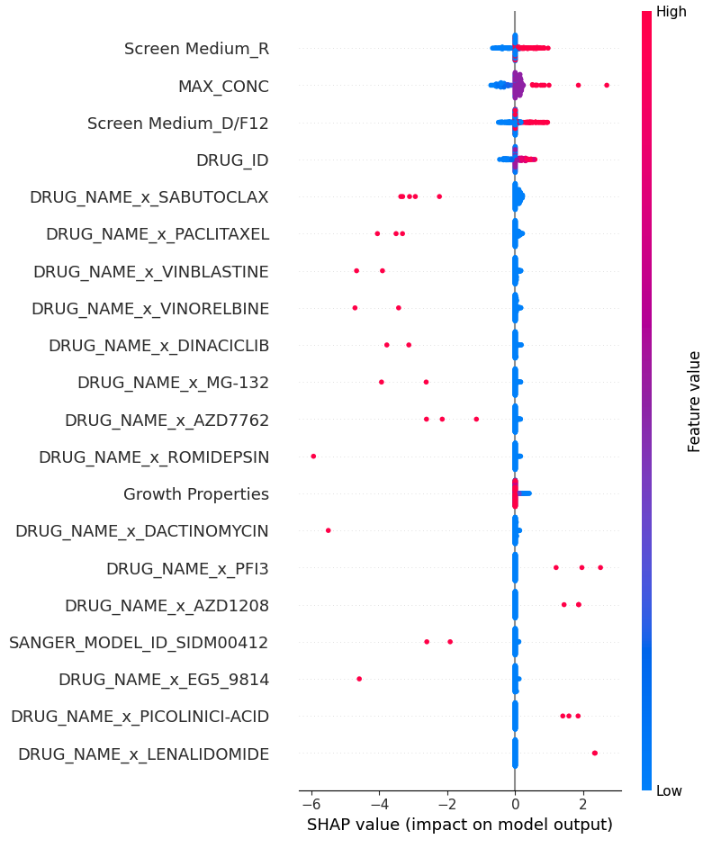
\includegraphics[width=1\textwidth]{figures/shap/shap_values.png}
    \caption{Shap summary plot with 200 examples. This one shows how the model behaves based on the values of its most representative variables.}
    \label{fig:shap_values}
\end{figure}

To interpret the image, it is important to note that all variables beginning with "DRUG\_NAME", "Screen Medium", or "SANER" have been one-hot encoded. This encoding explains the pattern of numerous blue dots and only a few red ones, indicating that the model primarily values the absence of these features. In contrast, the variable "DRUG\_ID" retains its original numerical values. Thus, the blue dots corresponding to these variables indicate that they are not present in the instance. For example, in the case of drug names, the blue dots represent those cases in which the drug in question has not been administered.

Figure~\ref{fig:shap_values} suggests that when the network detects that drugs such as Sabutoclax, Paclitaxel Vinblastine are recessed, the probability of predicting a low value for the \(LN\_IC_{50}\) variable increases, since all of them contribute to reducing the prediction value. Applying this knowledge to real life could mean that these drugs are more aggressive against cancer and therefore the amount needed is lower. In fact, according to several studies \cite{Hu2018Sabutoclax, DAguanno2020Bcl2}, Sabutoclax is mainly used in cases where the patient experiences some resistance to standard therapies.

Similarly, it can be seen that when the maximum concentration increases the model, so does the probability of predicting a high value for \(LN\_IC_{50}\).

Regarding the listed drugs, the presence of the first 9 appears to be associated with lower predictions for the \(LN\_IC_{50}\) variable, which is considered a favorable outcome for patients. Notably, one of the 20 most influential features is linked to the blood sample type. Its presence consistently contributes to lower \(LN\_IC_{50}\) values, reinforcing the hypothesis that genetic or biological factors, such as the type of sample, may significantly influence a patient's response to cancer treatments. This finding supports the broader theory that the human genome plays a crucial role in drug sensitivity.

The dependency plot for the variable SANGER\_MODEL\_ID\_SIDM00412, illustrated in Figure~\ref{fig:dependenceSanger}, reveals that, in the cases analysed by SHAP, when this specific blood sample is present, the value of the Growth Properties feature is never set to D/F12. This combination is associated with negative SHAP values for the target variable  \(LN\_IC_{50}\), suggesting that patients corresponding to this sample tend to require a lower dosage of medication. This may indicate a favorable drug sensitivity profile for this particular biological condition.

\begin{figure}[H]
    \centering
    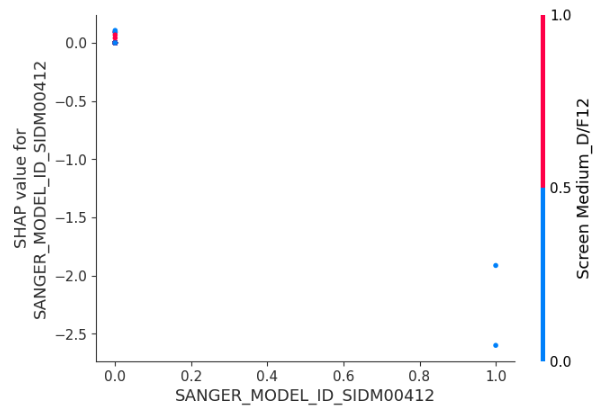
\includegraphics[width=1\textwidth]{figures/shap/dependence_plot_sanger.png}
    \caption{Dependence plot of variable SANGER\_MODEL\_ID\_SIDM00412 obtained using SHAP. Obtained by analysing 200 examples.}
    \label{fig:dependenceSanger}
\end{figure}